\documentclass{article}

\usepackage{gensymb}
\usepackage{graphicx}
\usepackage{float}

\begin{titlepage}
    \title{Assignment 2: Neural Networks \& Keras Intro}
    \author{BJ Bae}
    \date{\today}
\end{titlepage}

\begin{document}
\maketitle
\tableofcontents

\section{Introduction}
    The purpose of this assignment was to replicate the textbook's examples on 
    3 different types of neural networks (binary classification, 
    multiclass classification, and regression) and run further research on each 
    of the models. The binary classification example took the IMDB Movies dataset
    in Keras to determine whether or not a movie would have positive or negative reviews 
    based on its characteristics. The multiclass classification example took the Reuters dataset
    in Keras to classify a topic based on a short bit of text. The regression example used the 
    Boston Housing dataset in Keras to predict median home prices in a Boston suburb 
    in the 1970s given the neighborhood characteristics. None of these problems are particularly 
    new or difficult but they provided good practice to develop a strategy to handle 
    different types of problems.
    
    Another part of the assignment was to also pick out a dataset to analyze 
    and create a neural network through the Keras library. The dataset that was
    used for this part of the assignment was Seoul's bicycle sharing dataset from UCI.
    The goal for this part of the assignment was to predict how many bicycles would be used in 
    bicycle sharing system at a certain time given particular characteristics about a day like
    temperature, humidity, holiday, etc.


\section{Discussion}
    The bicycle sharing dataset has information about date, 
    temperature (\degree C), humidity (\%), wind speed (m/s), 
    visibility (10m),  dew point temperature (\degree C), 
    solar radiation (MJ/m\textsuperscript{2}), 
    rainfall (mm), snowfall (cm), season, hour of day, functioning day , holiday, 
    and rented bike count.
    The functioning day field is a boolean value that represented if the bike 
    sharing system was functioning or under repair.
    The holiday field is also a boolean value that represented if that day was 
    a holiday or not.
    For data cleaning before feeding the data into the models, the date field was 
    removed to not have any identifiers on specific dates that the model could have 
    access to for training, although seasonality and time of day were both important fields
    that the model could train on. The data points where the non-functioning day field
    was true and the entire field of functioning day were also removed. The model could use this field to predict a drop in 
    bicycles rented with 100\% correlation with this variable, which was not the 
    intended purpose of this exercise. With all the non-functioning days removed, the column would 
    only contain functioning days which would be useless for the model so the column was also dropped. 
    However, the data points on holidays were not dropped.While a drop in bicycle rentals 
    might be inferred, it is a more natural occurence and it is not immediately clear what 
    type of effect hoidays might have on bike rentals. This variable might also aid the model 
    in describing the anomalies that happen during holidays.

    The season, hour of day, and holiday fields were all one hot encoded, while the rest of the 
    continous predictors were standardized.


\section{Methods}
    There were a couple different models that were created in the process of finding the best model in predicting the most accurate
    bicycle sharing rental rate estimate. 

    All the models used a 20\% dropout layer between each hidden layer. All the loss functions were 
    using mean squared error with the adam optimizer and also displaying the mean absolute error metric.

    \begin{figure}[H]
        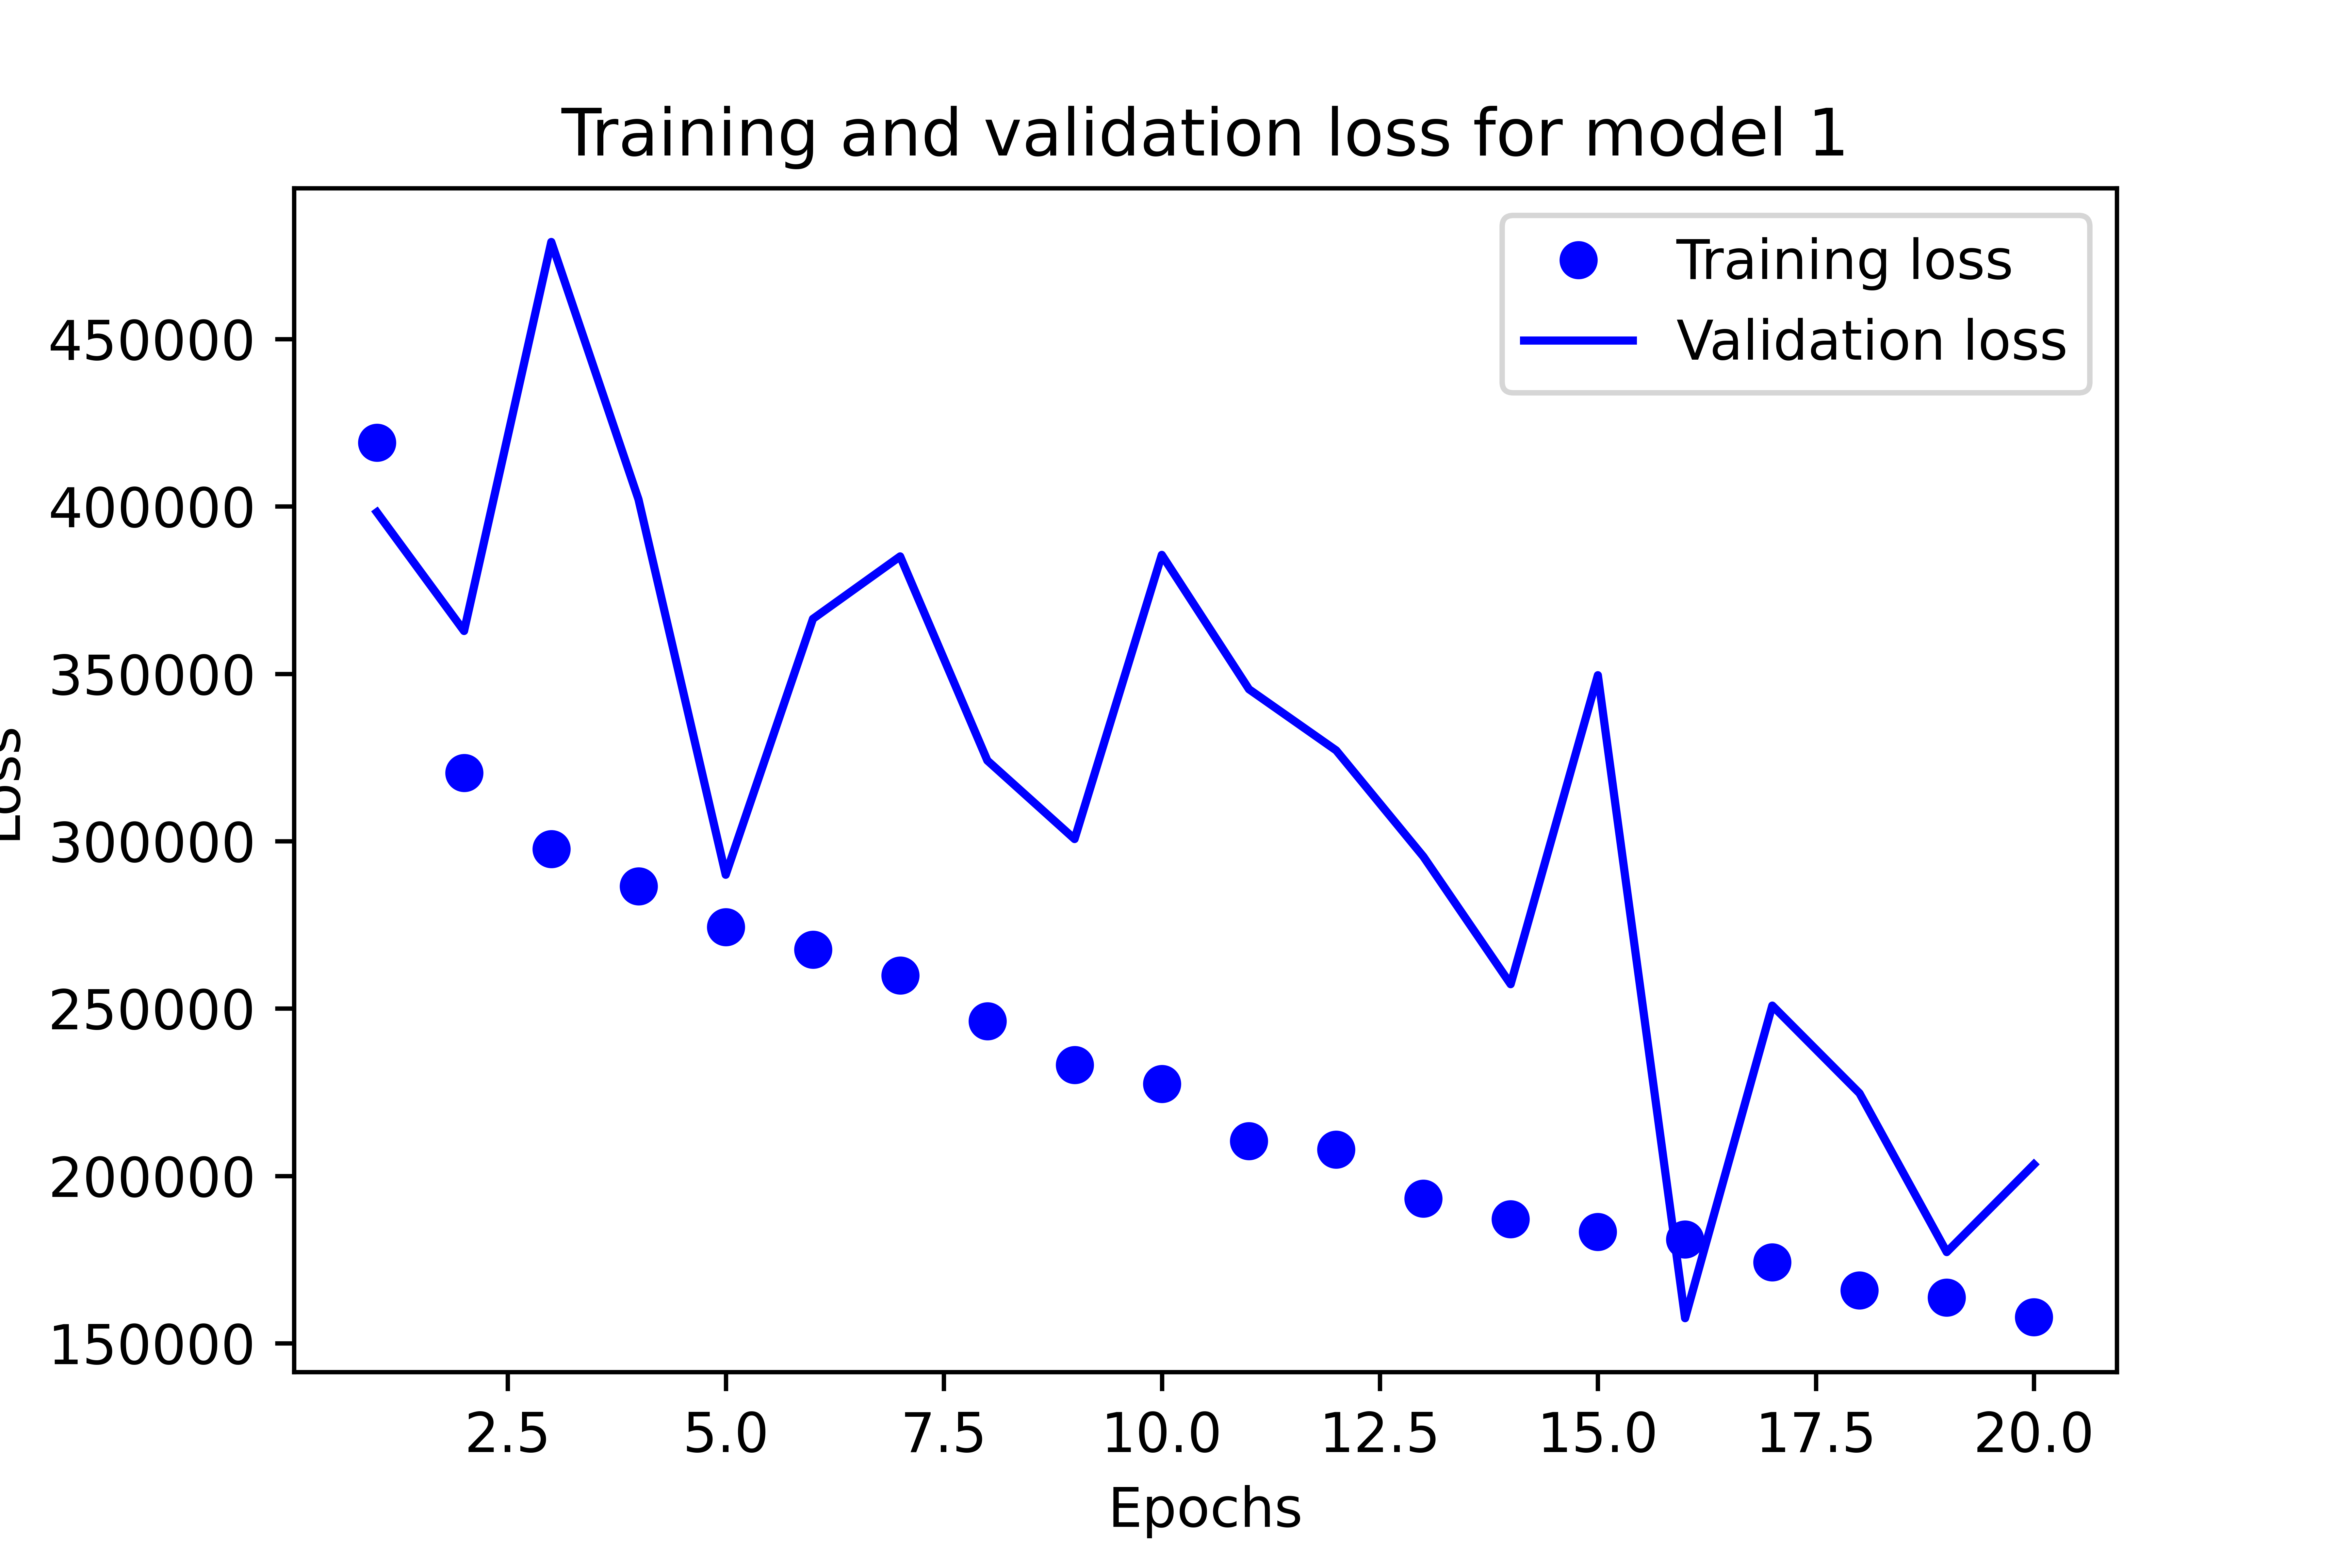
\includegraphics[width=\linewidth]{images/model1.png}
    \end{figure}
    The first model used a 3 layer 8-8-1 hidden layer output structure with a batch size of 1.
    It resulted in very high loss and big spikes in the validation loss, but there was a noticeable 
    negative slope in both training and validation losses, meaning that the model was underfitting.
    
    \begin{figure}[H]
        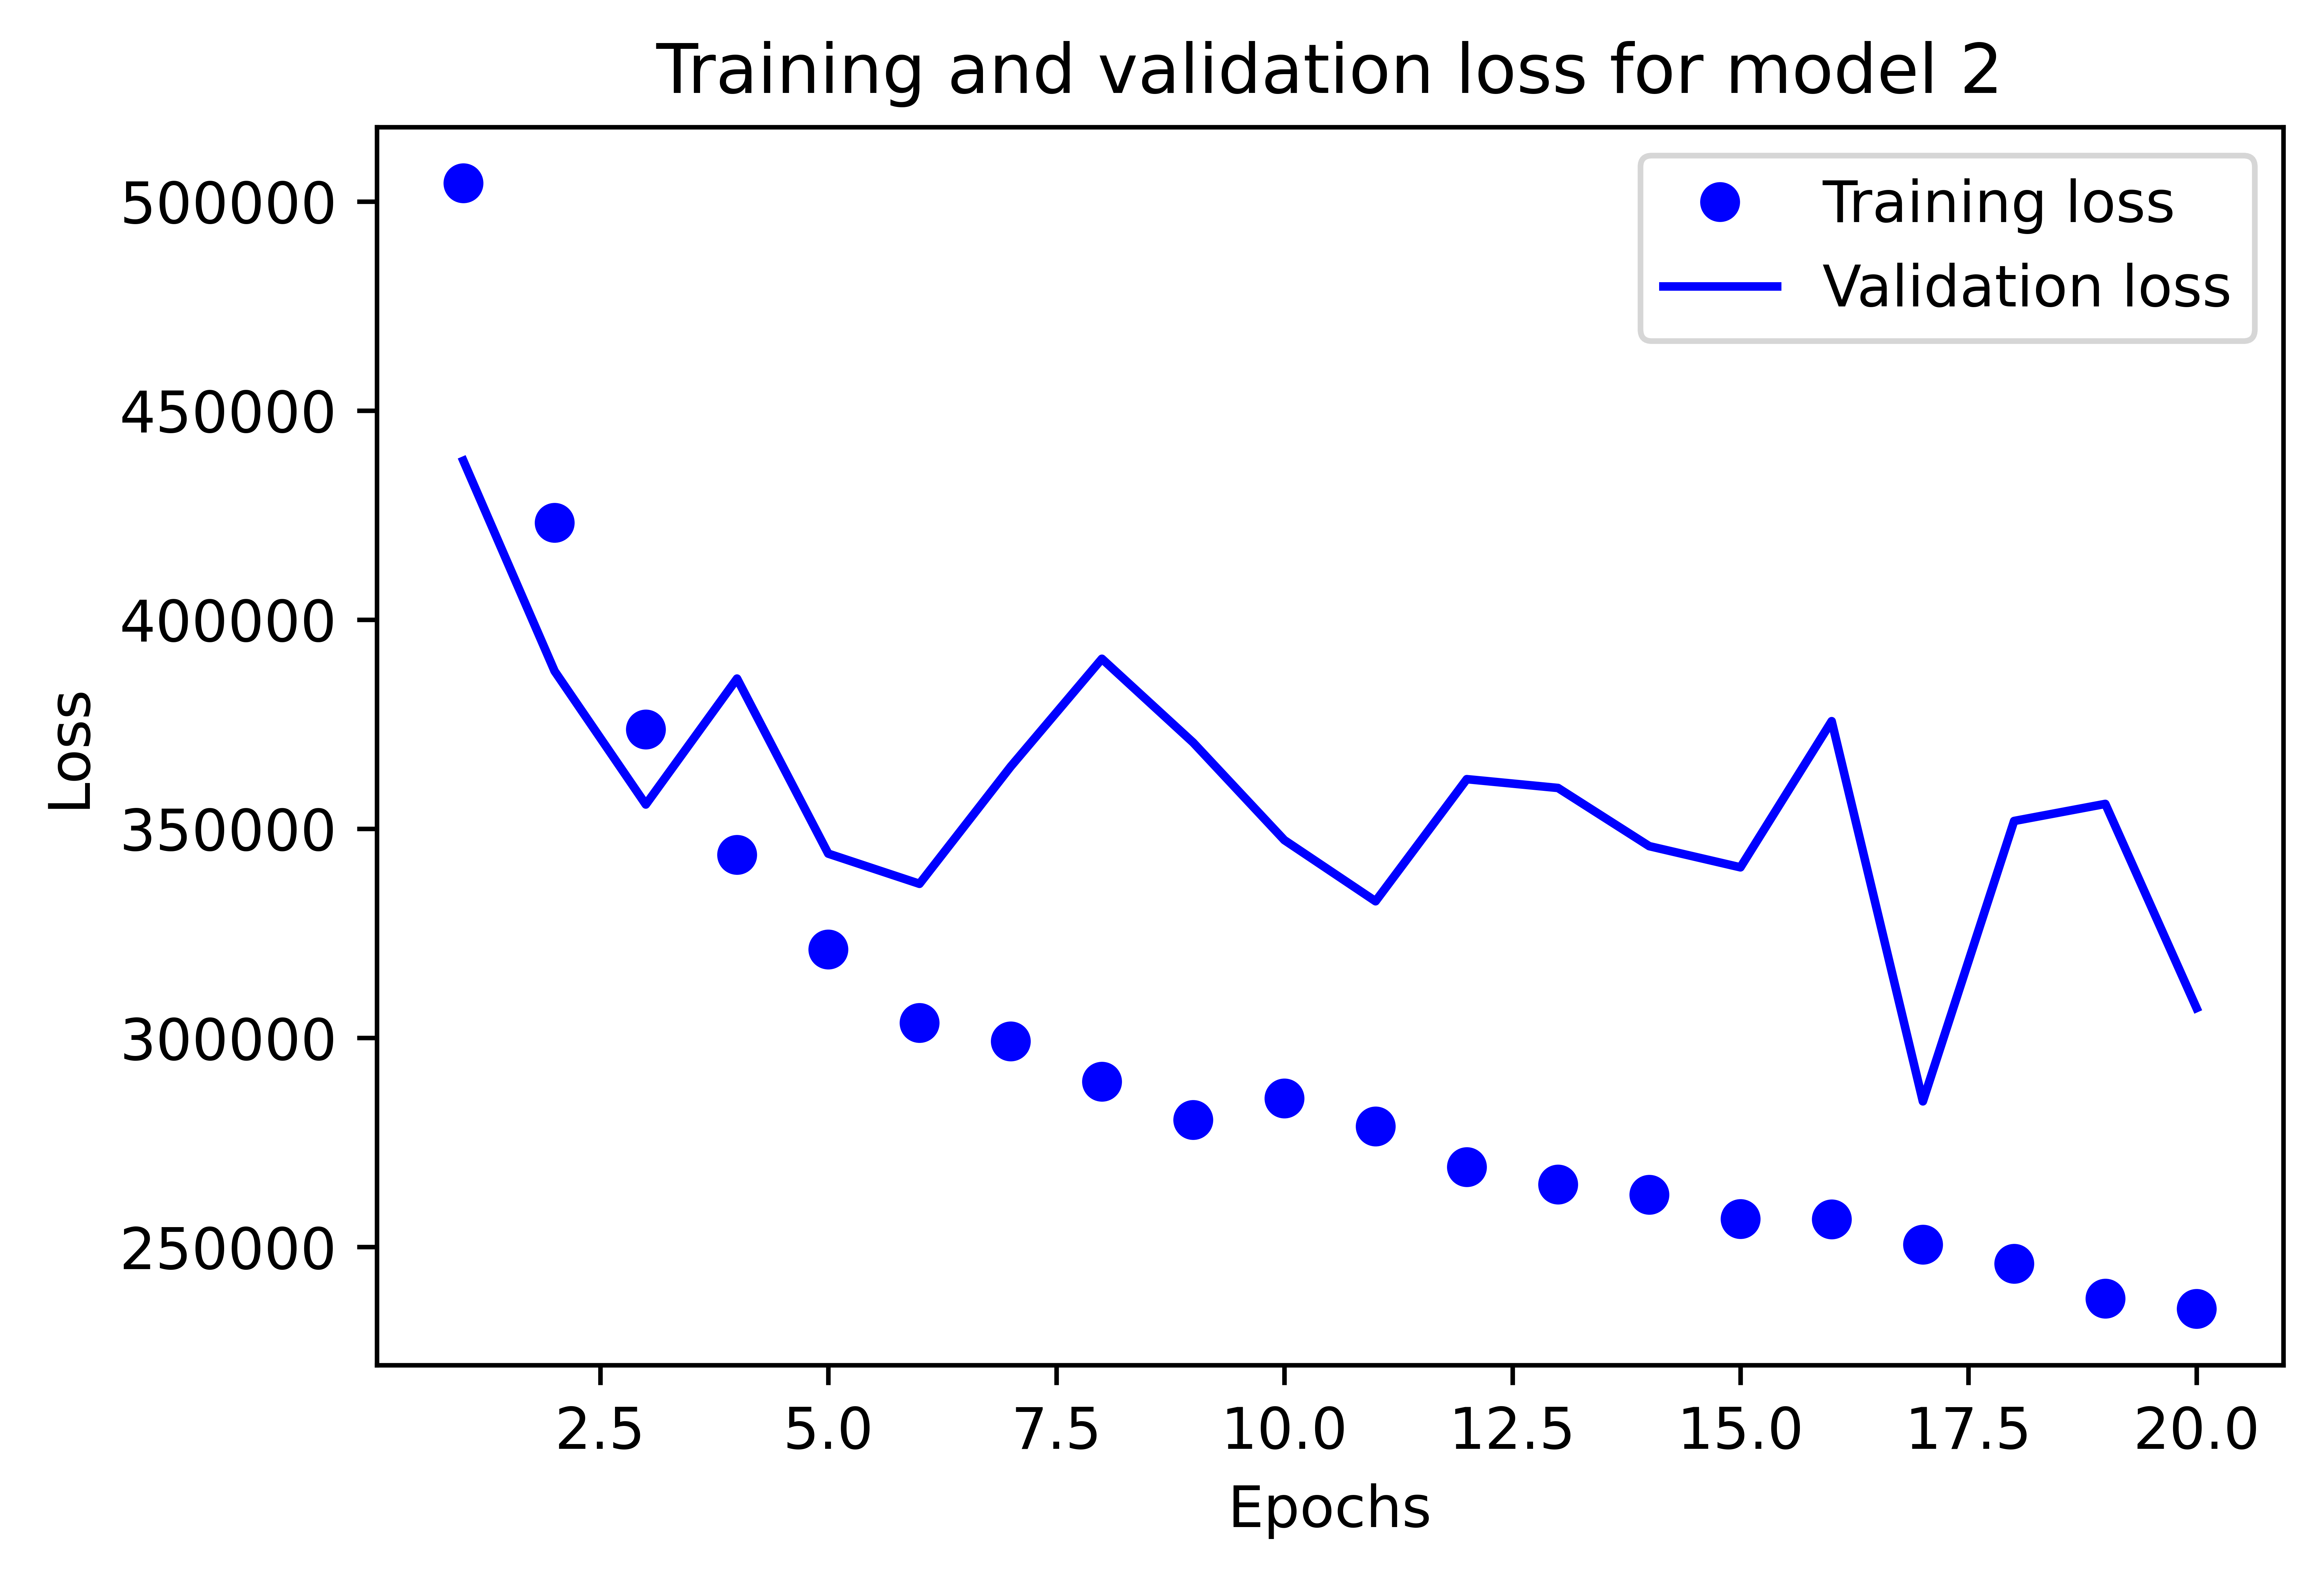
\includegraphics[width=\linewidth]{images/model2.png}
    \end{figure}
    Model 2 used the same structure as model 1, but with a higher batch size of 10 to mitigate the large spikes in the validation loss. While 
    losses went up it solved the instability problem of the validation loss.

    \begin{figure}[H]
        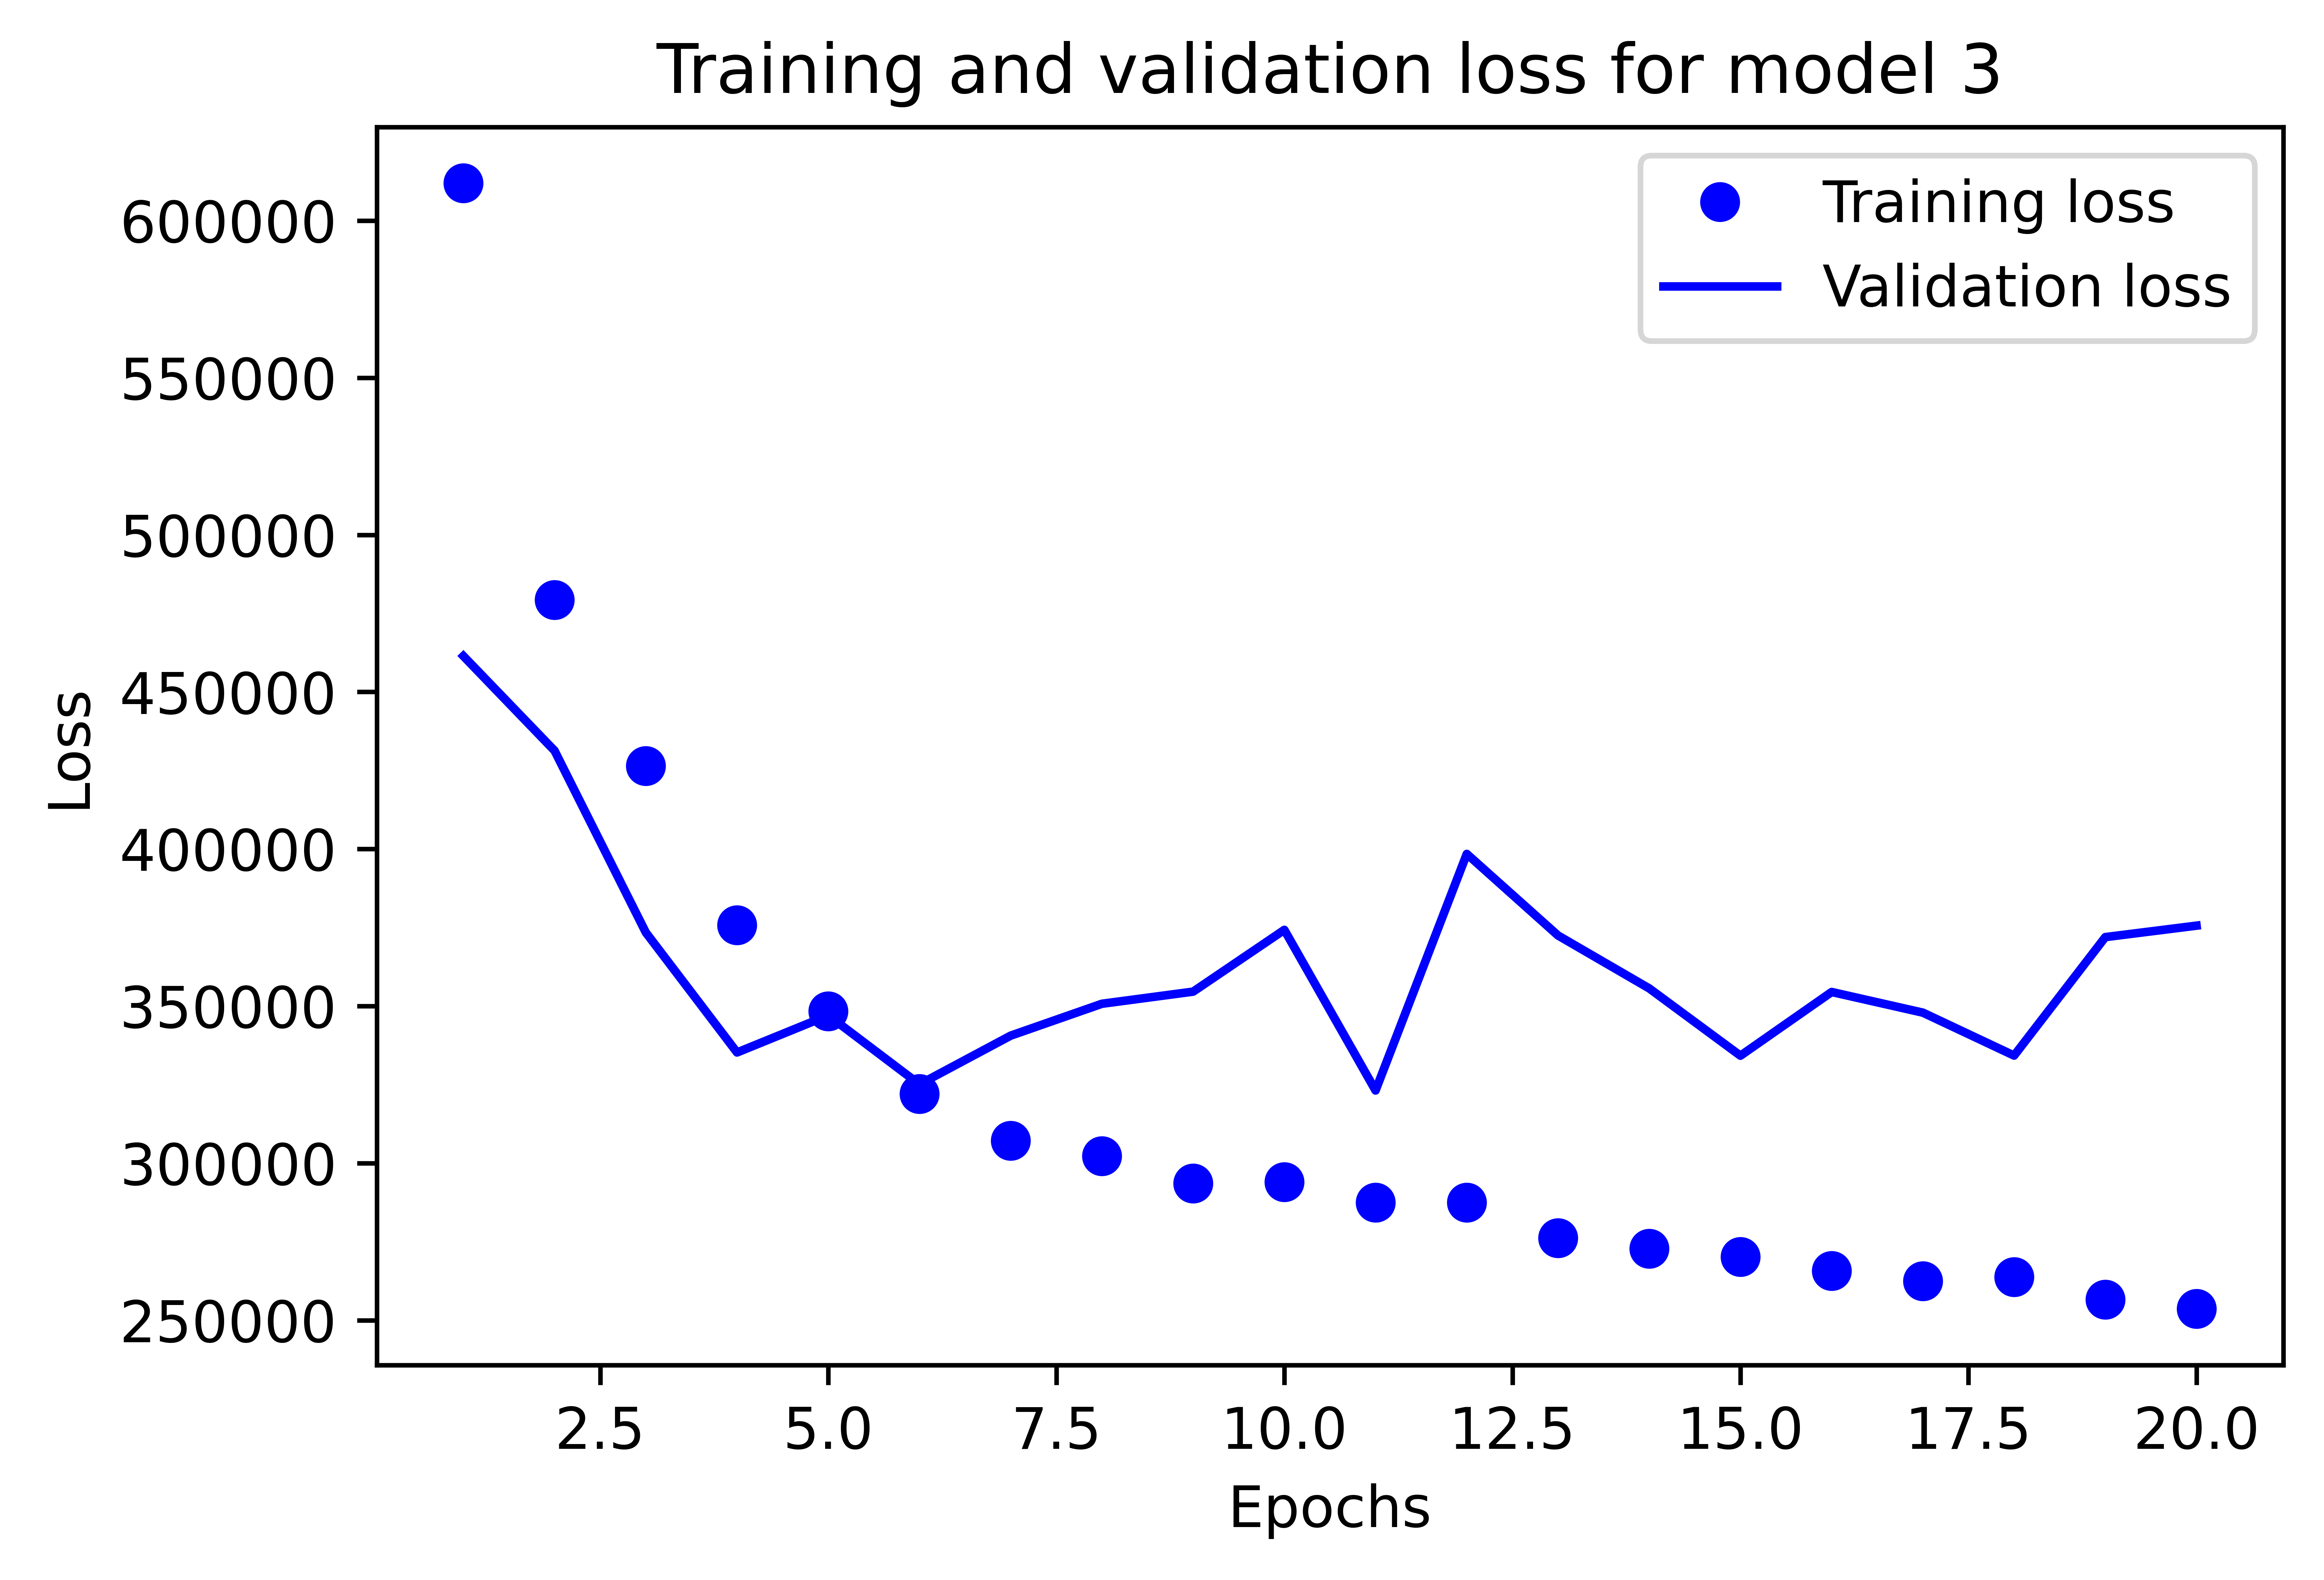
\includegraphics[width=\linewidth]{images/model3.png}
    \end{figure}
    Model 3 modified model 2 by increasing the batch size to 20, but the change made the stable validation loss worse and the relative 
    training loss the same.

    \begin{figure}[H]
        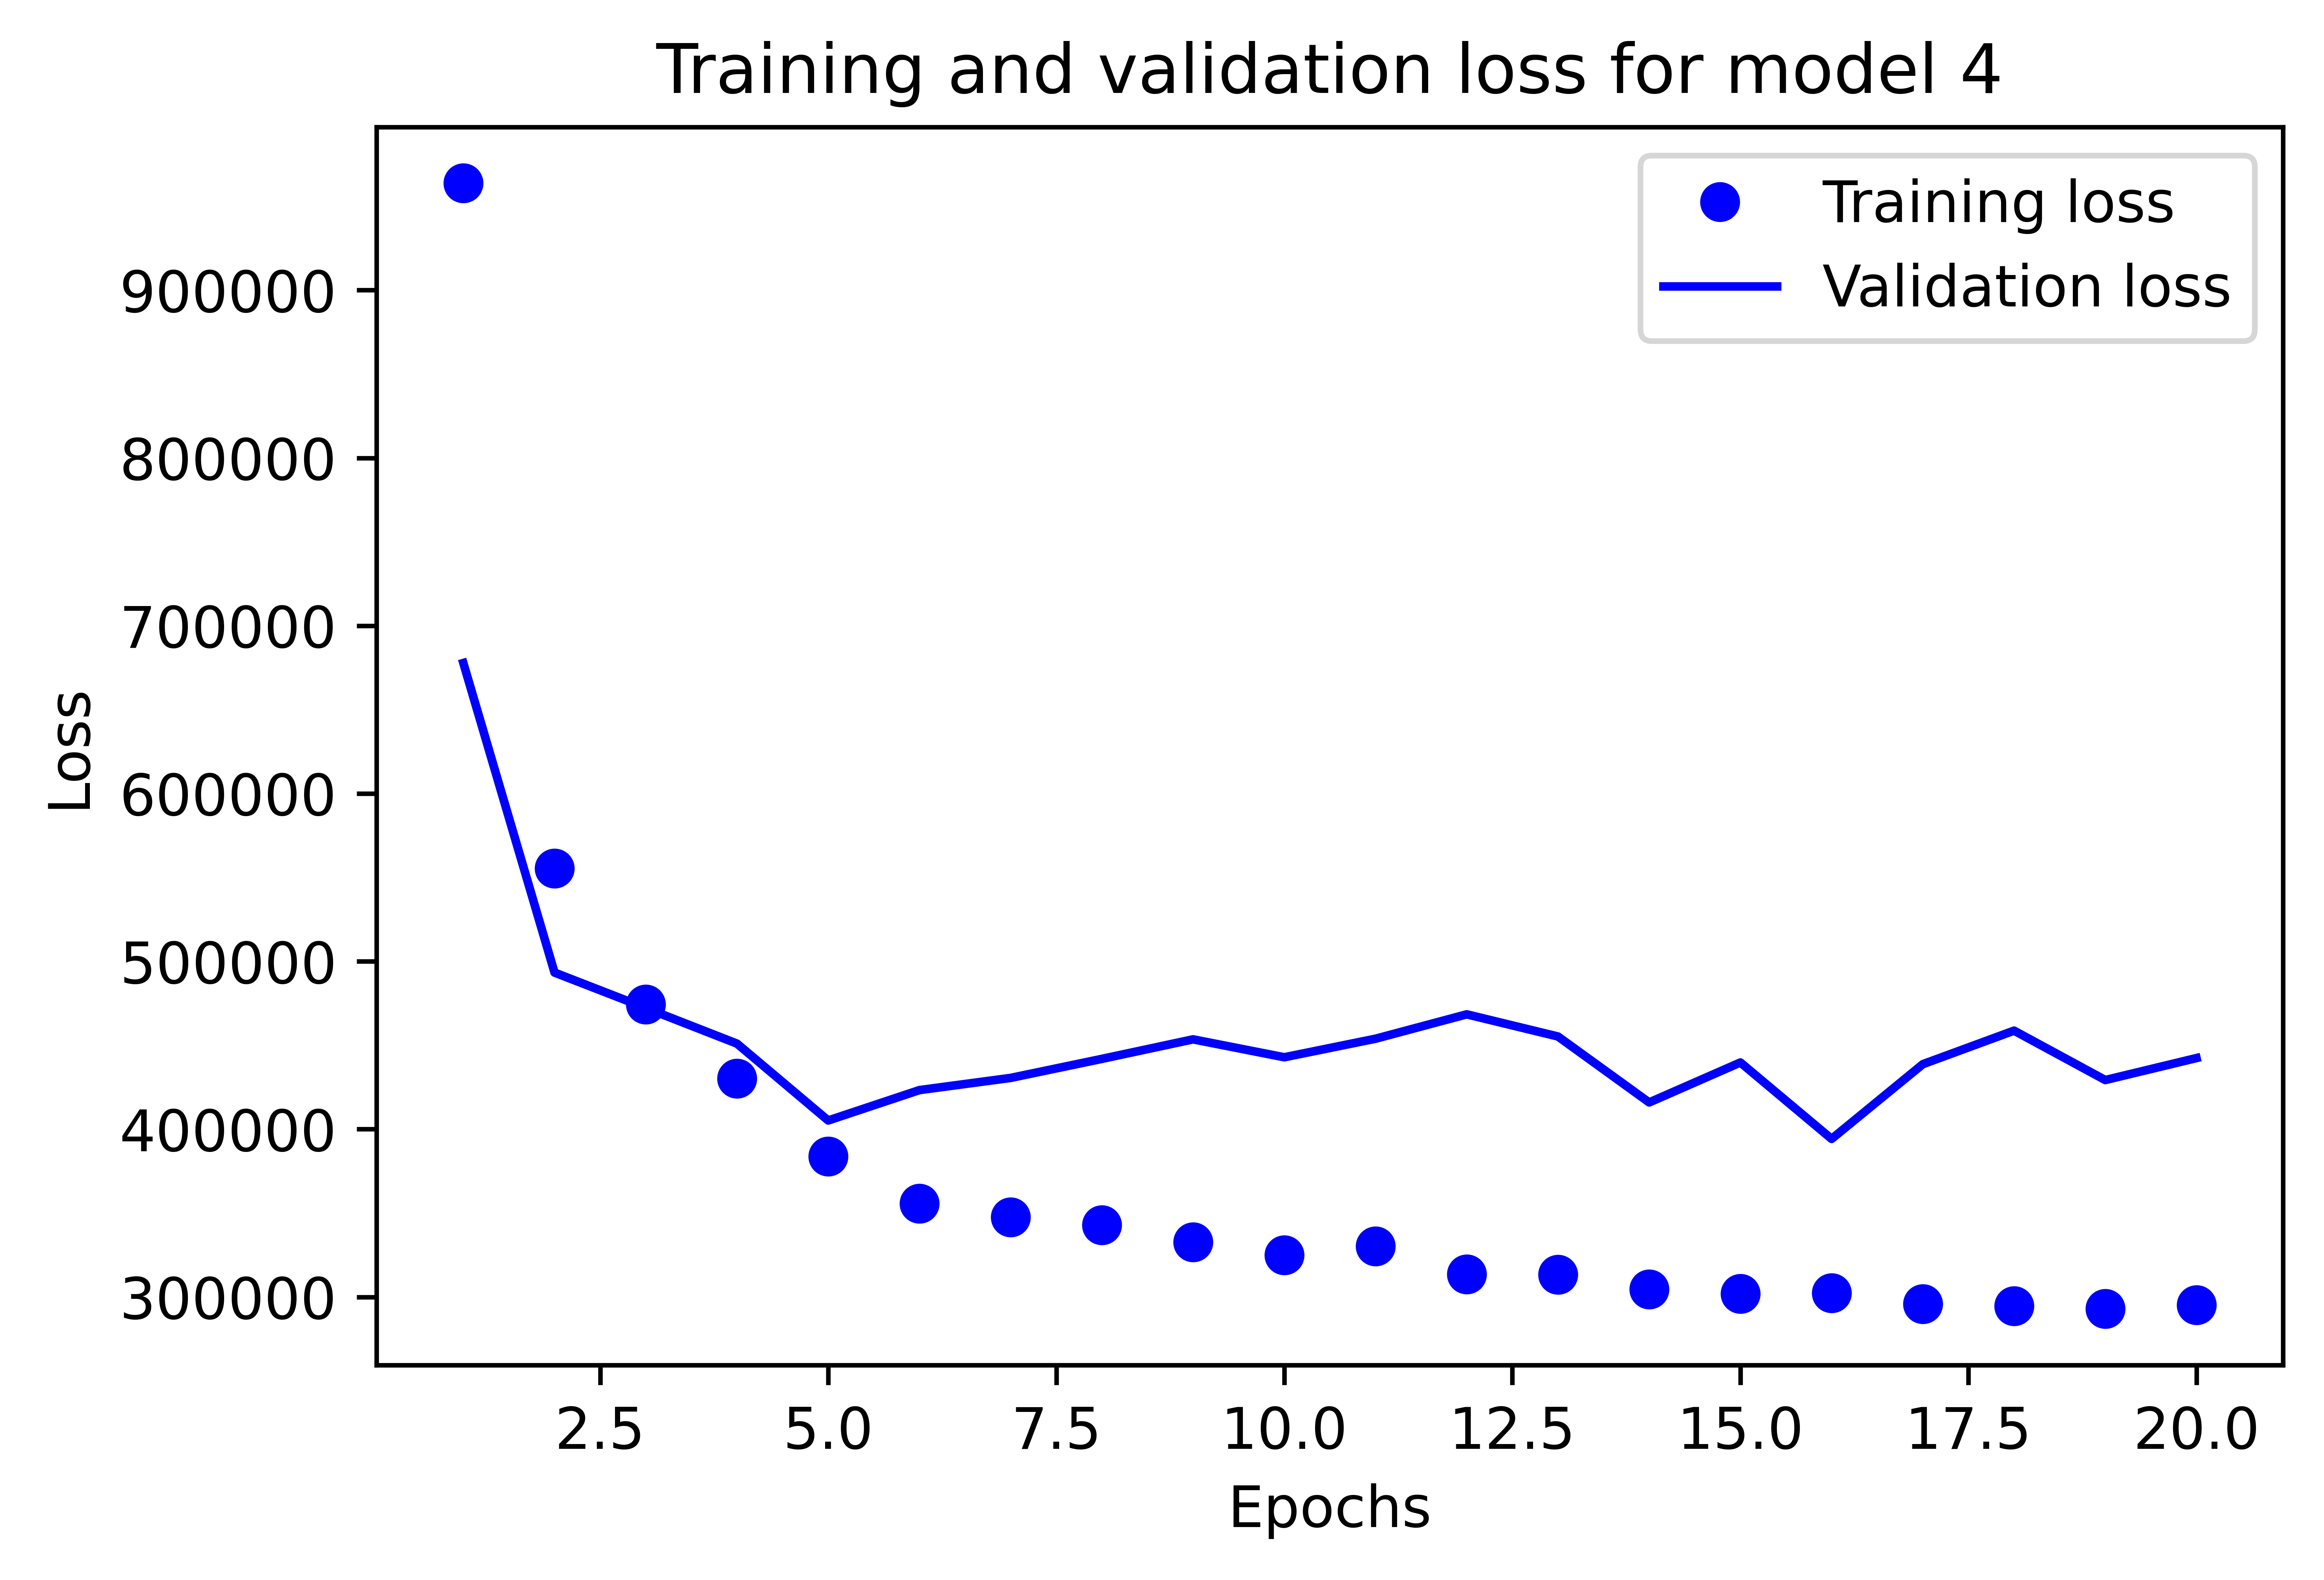
\includegraphics[width=\linewidth]{images/model4.png}
    \end{figure}
    Model 4 kept the batch size of 20 but added one more layer making it an 8-8-8-1 structure to increase model complexity. 
    While this looked like the validation loss was overfitting, it seemed that the loss was unchanging through the epochs. 
    This was confusing, so instead of increasing the depth of the neural network, the next iteration of the model added 
    more width instead.

    \begin{figure}[H]
        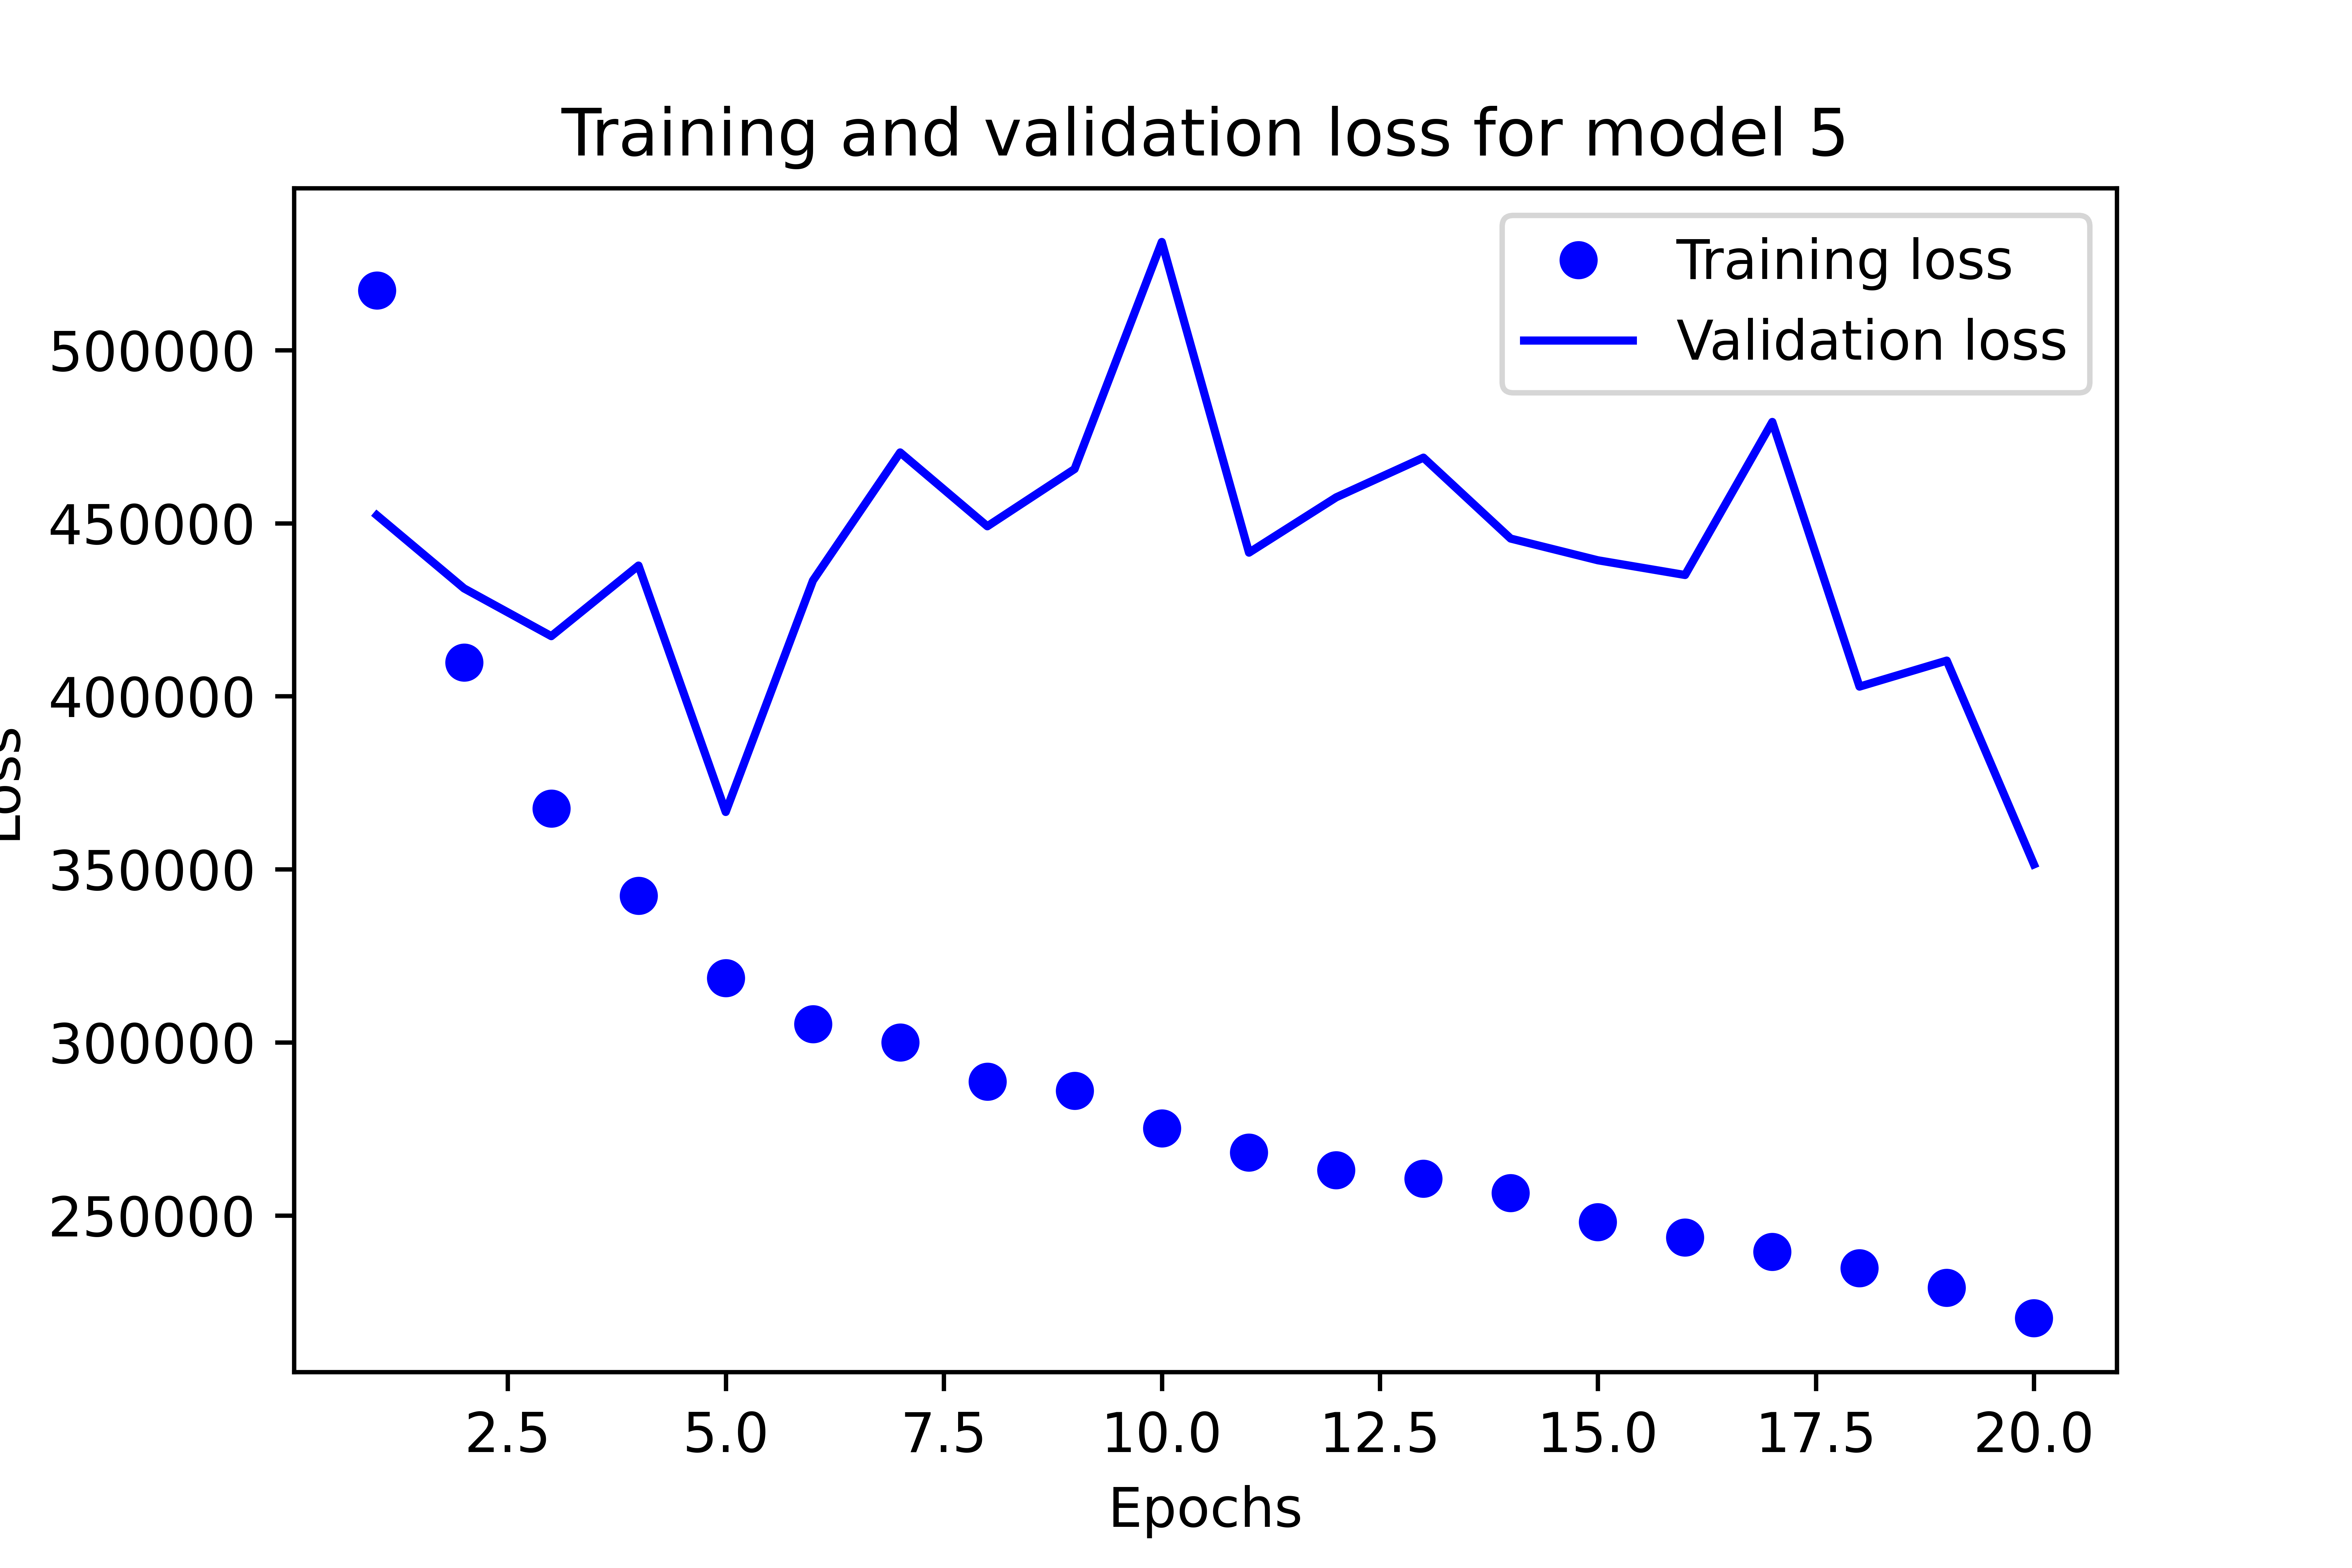
\includegraphics[width=\linewidth]{images/model5.png}
    \end{figure}
    Model 5 built off of the 8-8-8-1 structure to a 16-16-16-1. This model completely overfit and was not the right direction. 
    One reason that was hypothesized was because the input layer of 35 features were being bottlenecked by the first 16 unit hidden layer.

    \begin{figure}[H]
        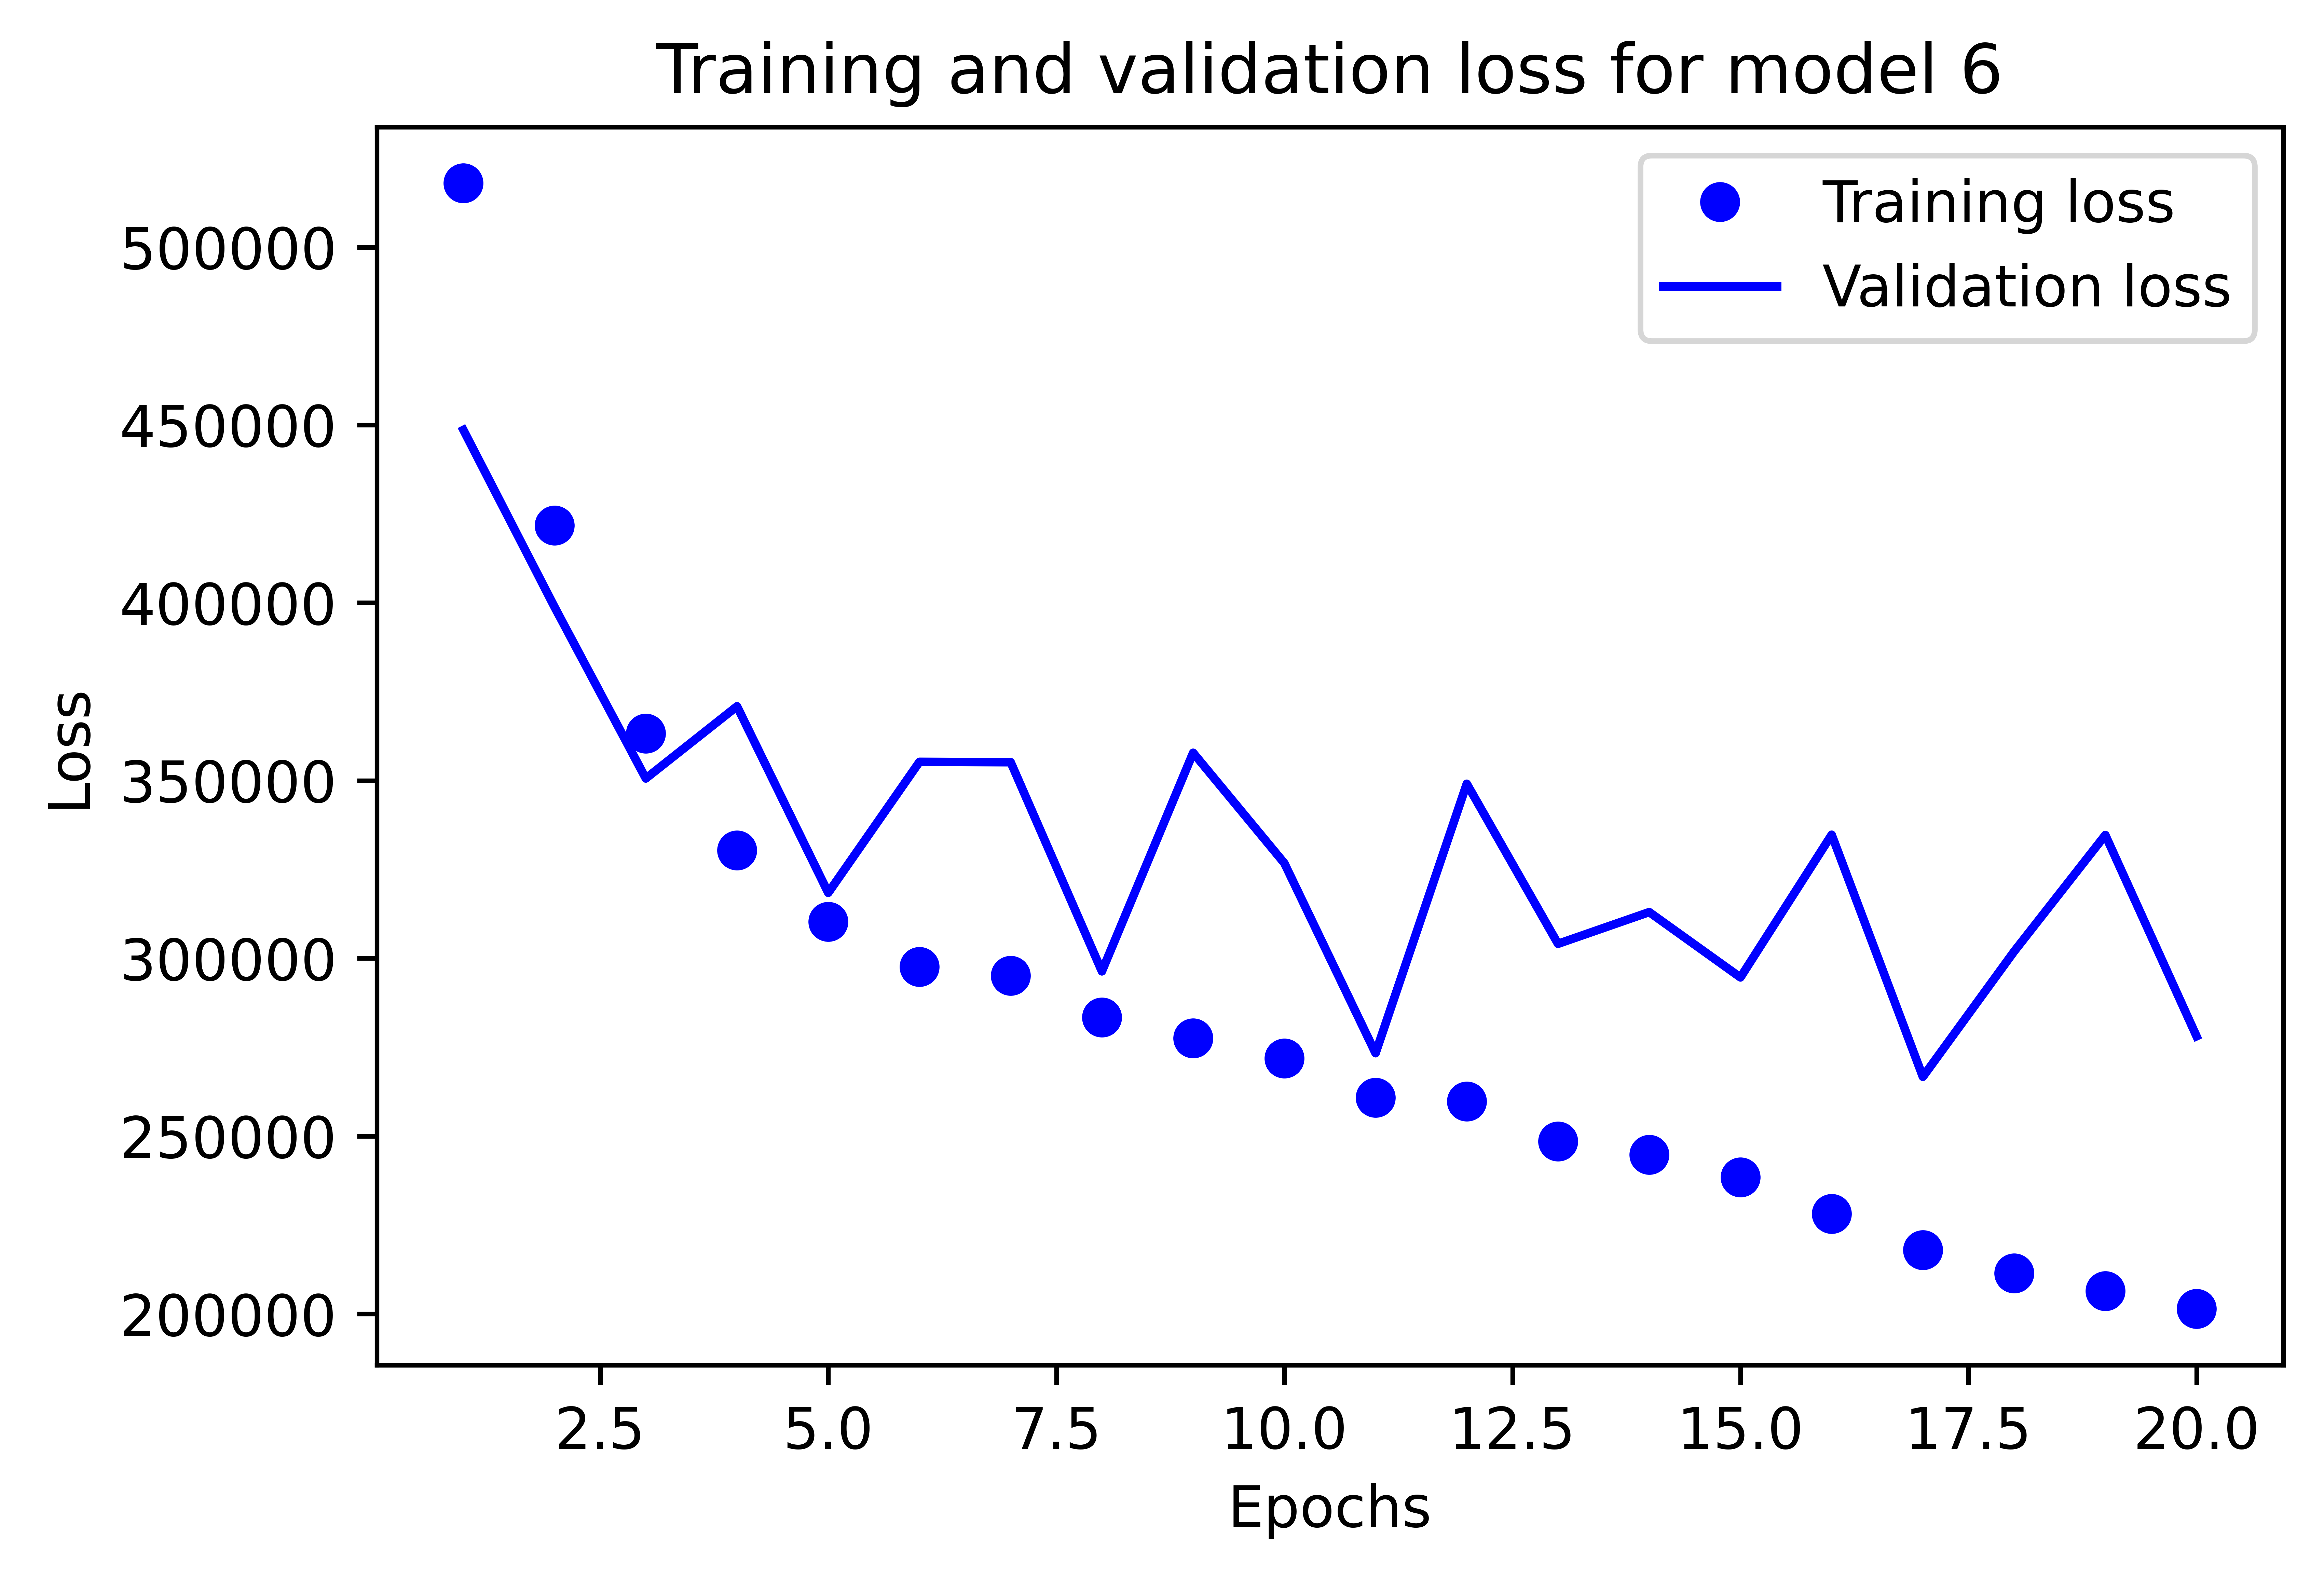
\includegraphics[width=\linewidth]{images/model6.png}
    \end{figure}
    To fix model 5's overfitting, model 6 made the first hidden layer 64 units (64-16-16-1). This helped stop the overfitting and decreased overall 
    loss to the lowest levels.

    \begin{figure}[H]
        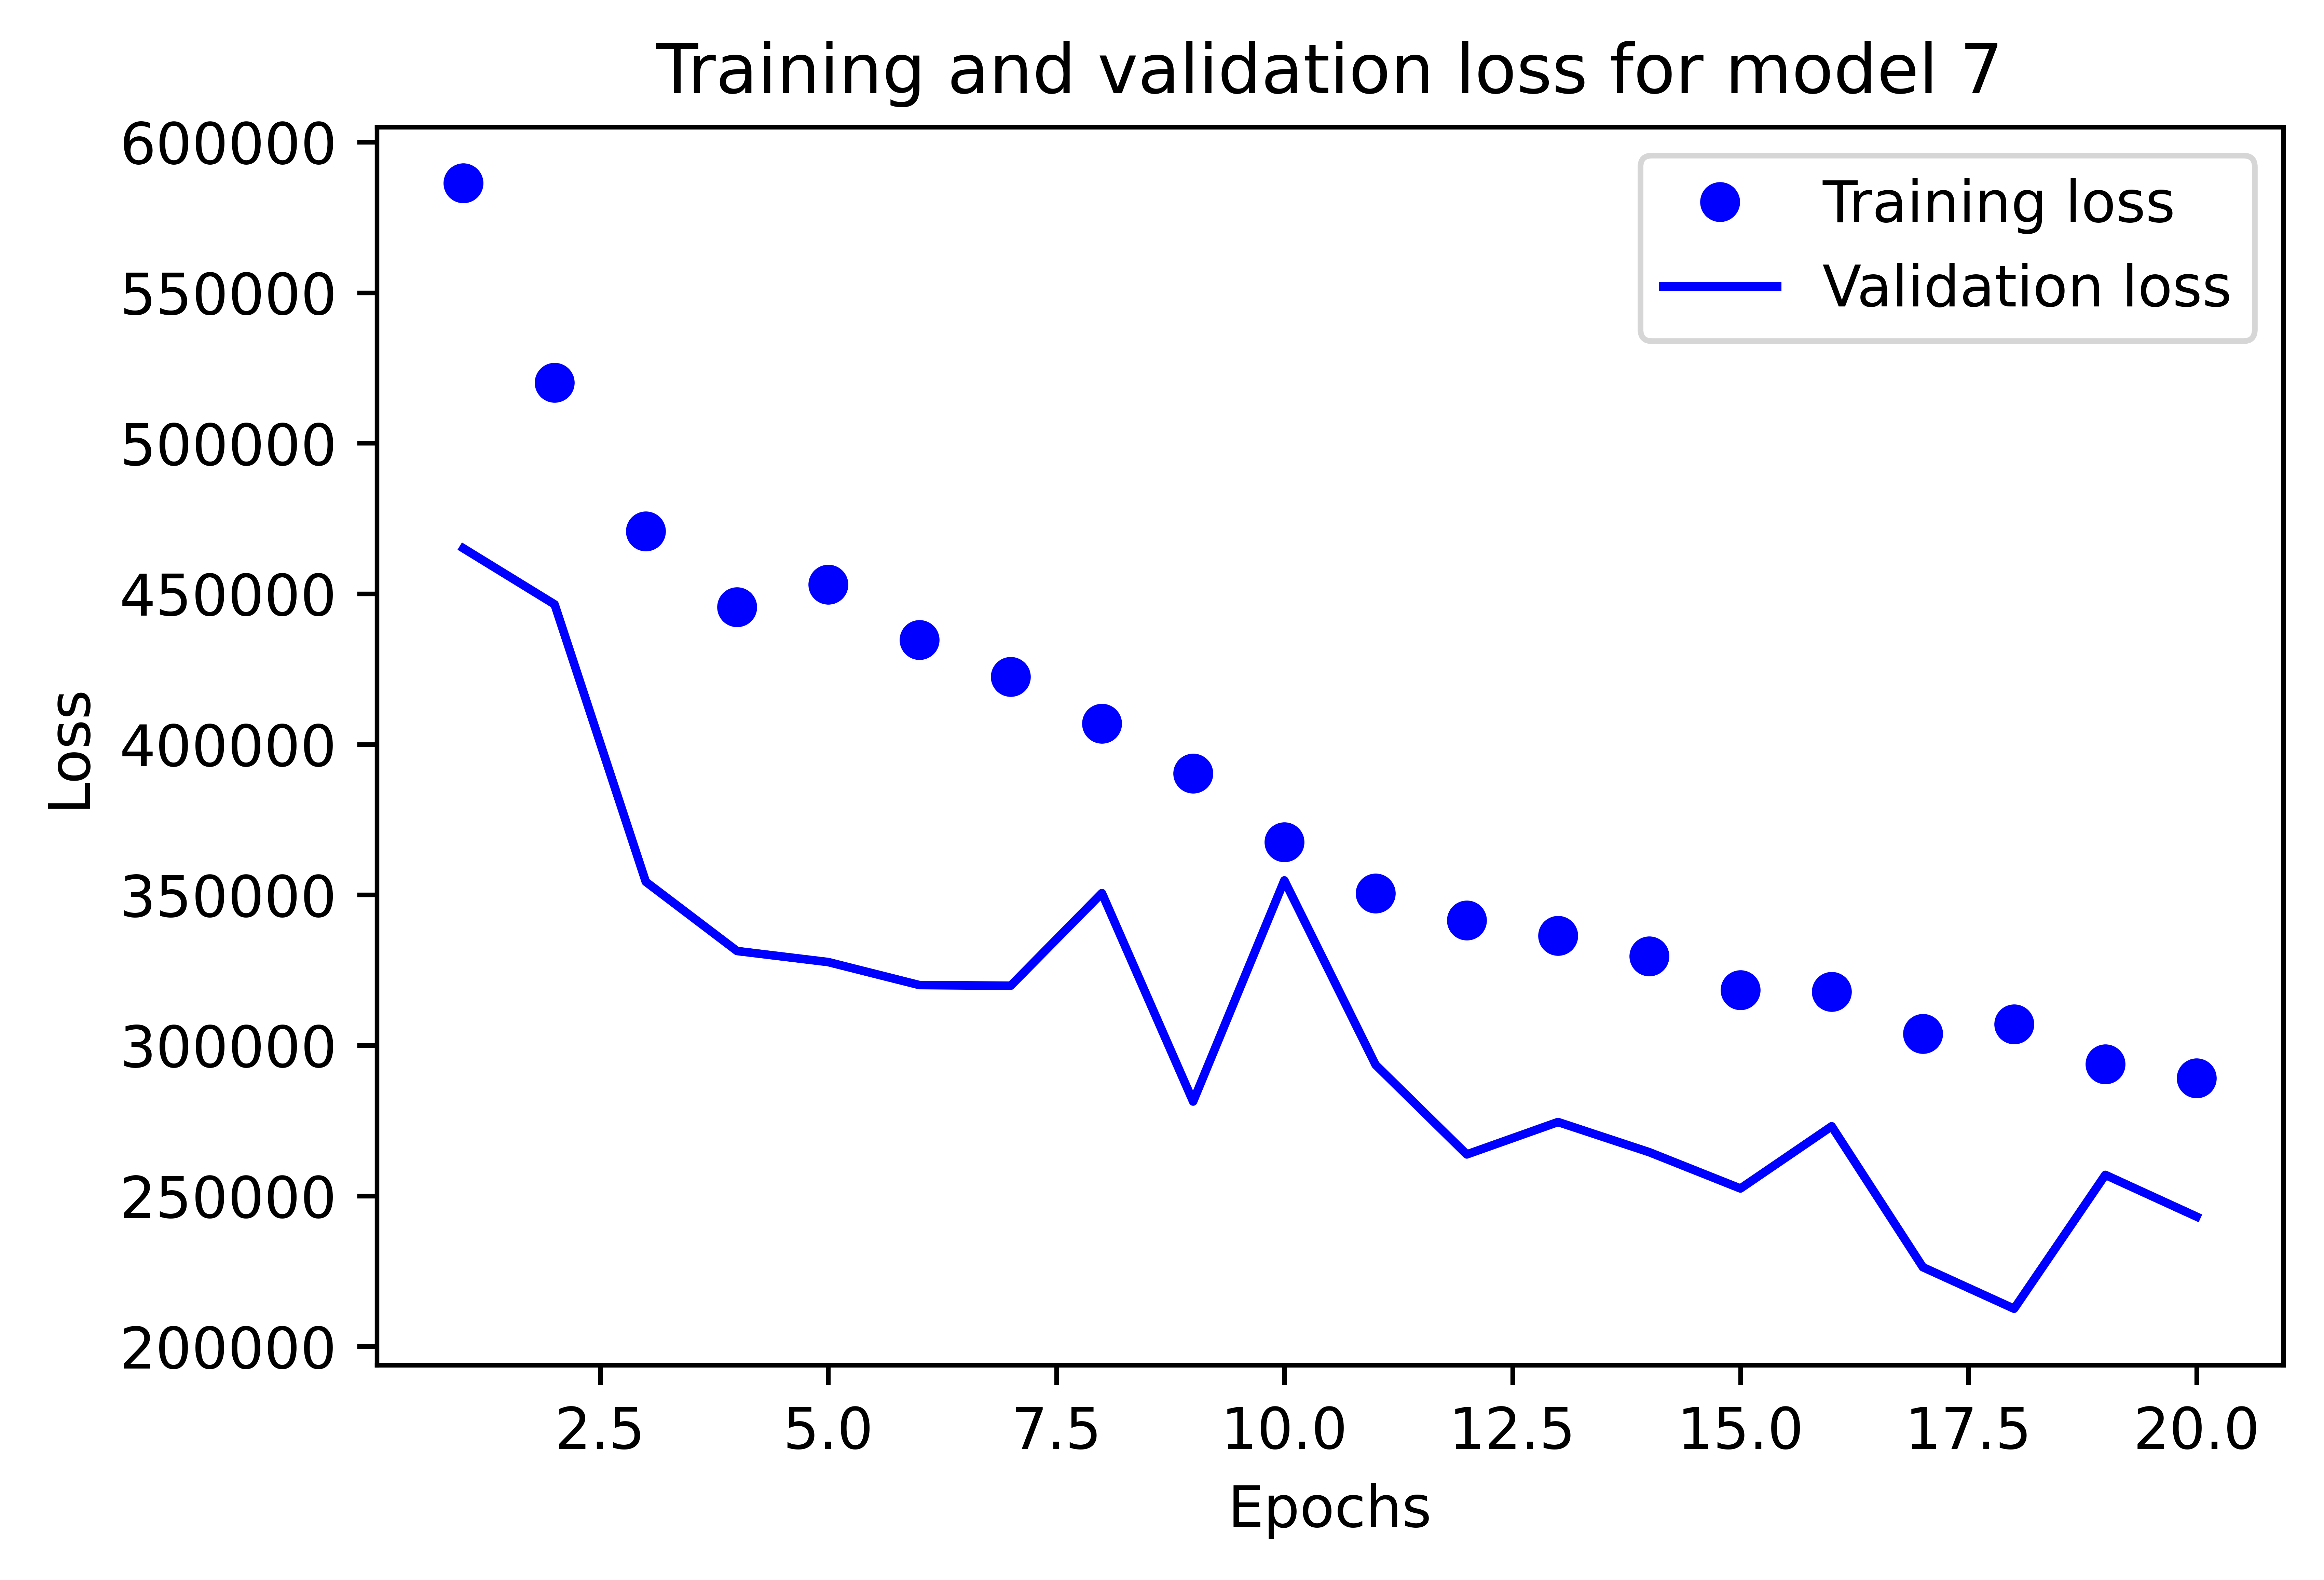
\includegraphics[width=\linewidth]{images/model7.png}
    \end{figure}
    Following up on model 6's more asymetrical width structure, model 7 made the second to last hidden layer more narrow, down from 16 to 8 units 
    (64-16-8-1). This significantly helped bring the validation loss. The validation loss was below the training loss. One of the explainations 
    for this was that the training data goes through the dropout layers which might contribute to higher loss that the validation data doesn't go 
    through. Since the loss was so low, the next model adds complexity to gain lower loss before it overfits.

    \begin{figure}[H]
        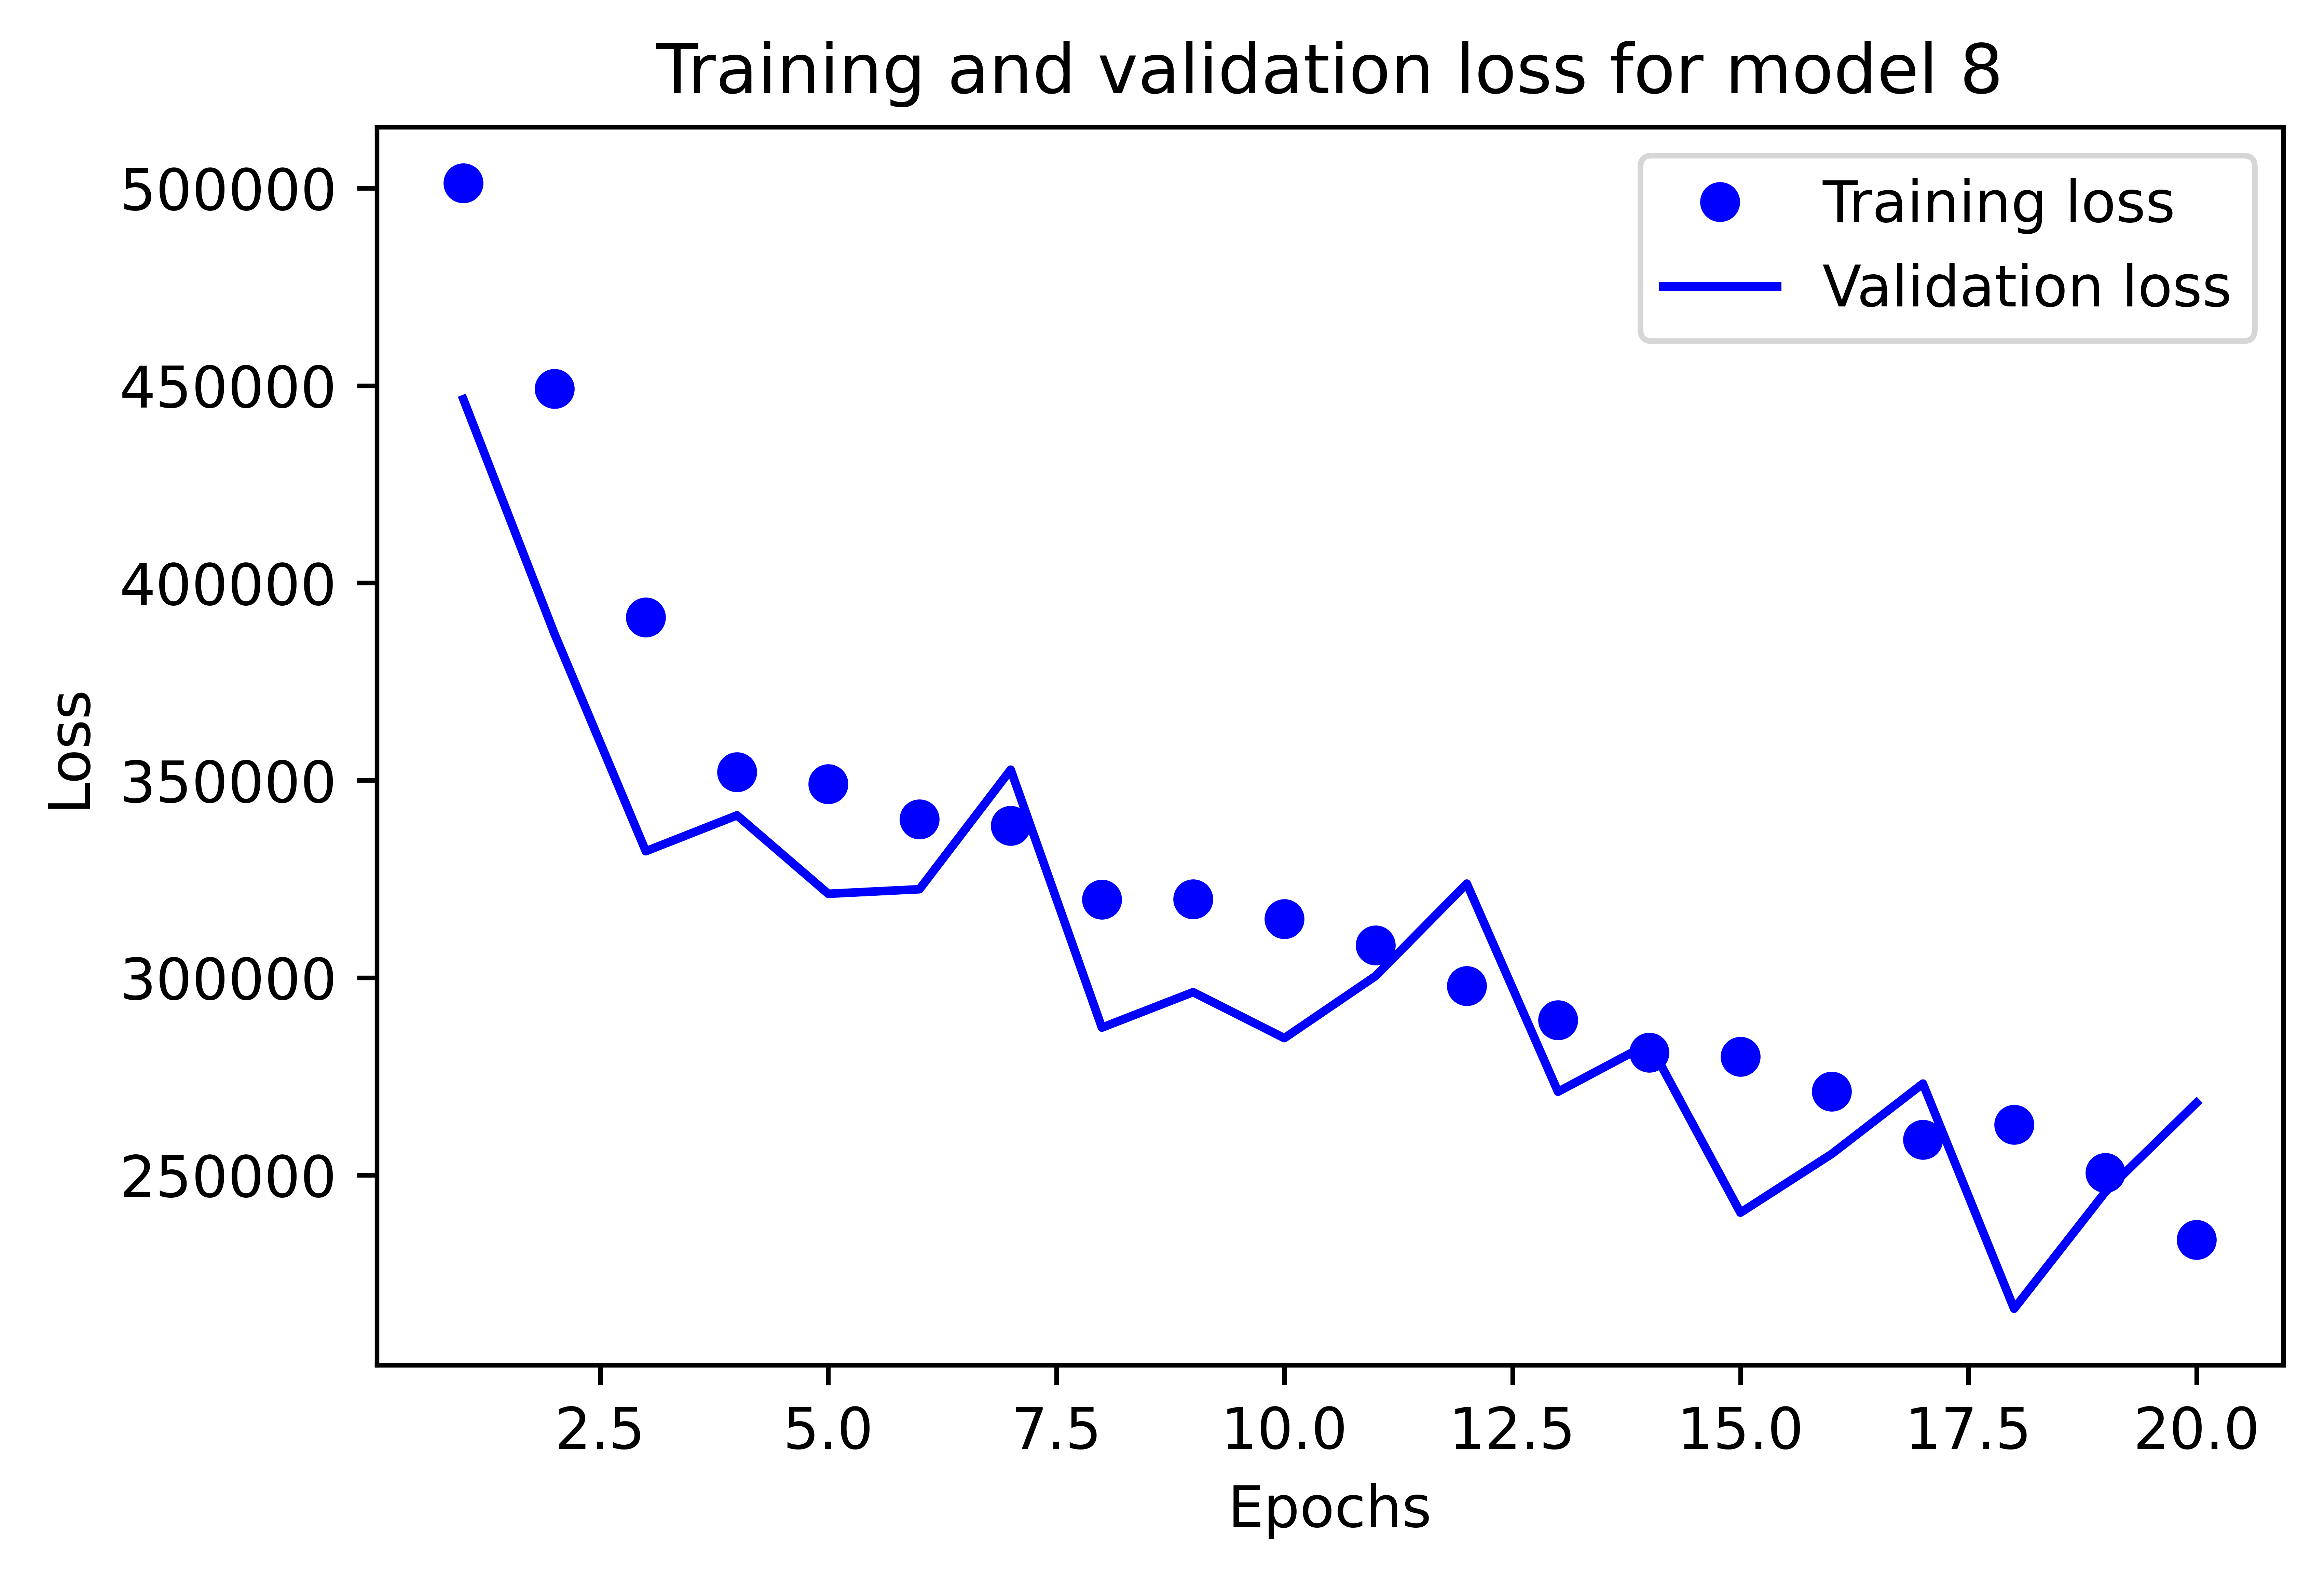
\includegraphics[width=\linewidth]{images/model8.png}
    \end{figure}
    Model 8 adds another hidden layer making the structure 64-32-16-8-1. For all these past models, unless stated otherwise, has no 
    change to the batch sizes or any other parameter. This model performed even better and continued to not overfit.

    \begin{figure}[H]
        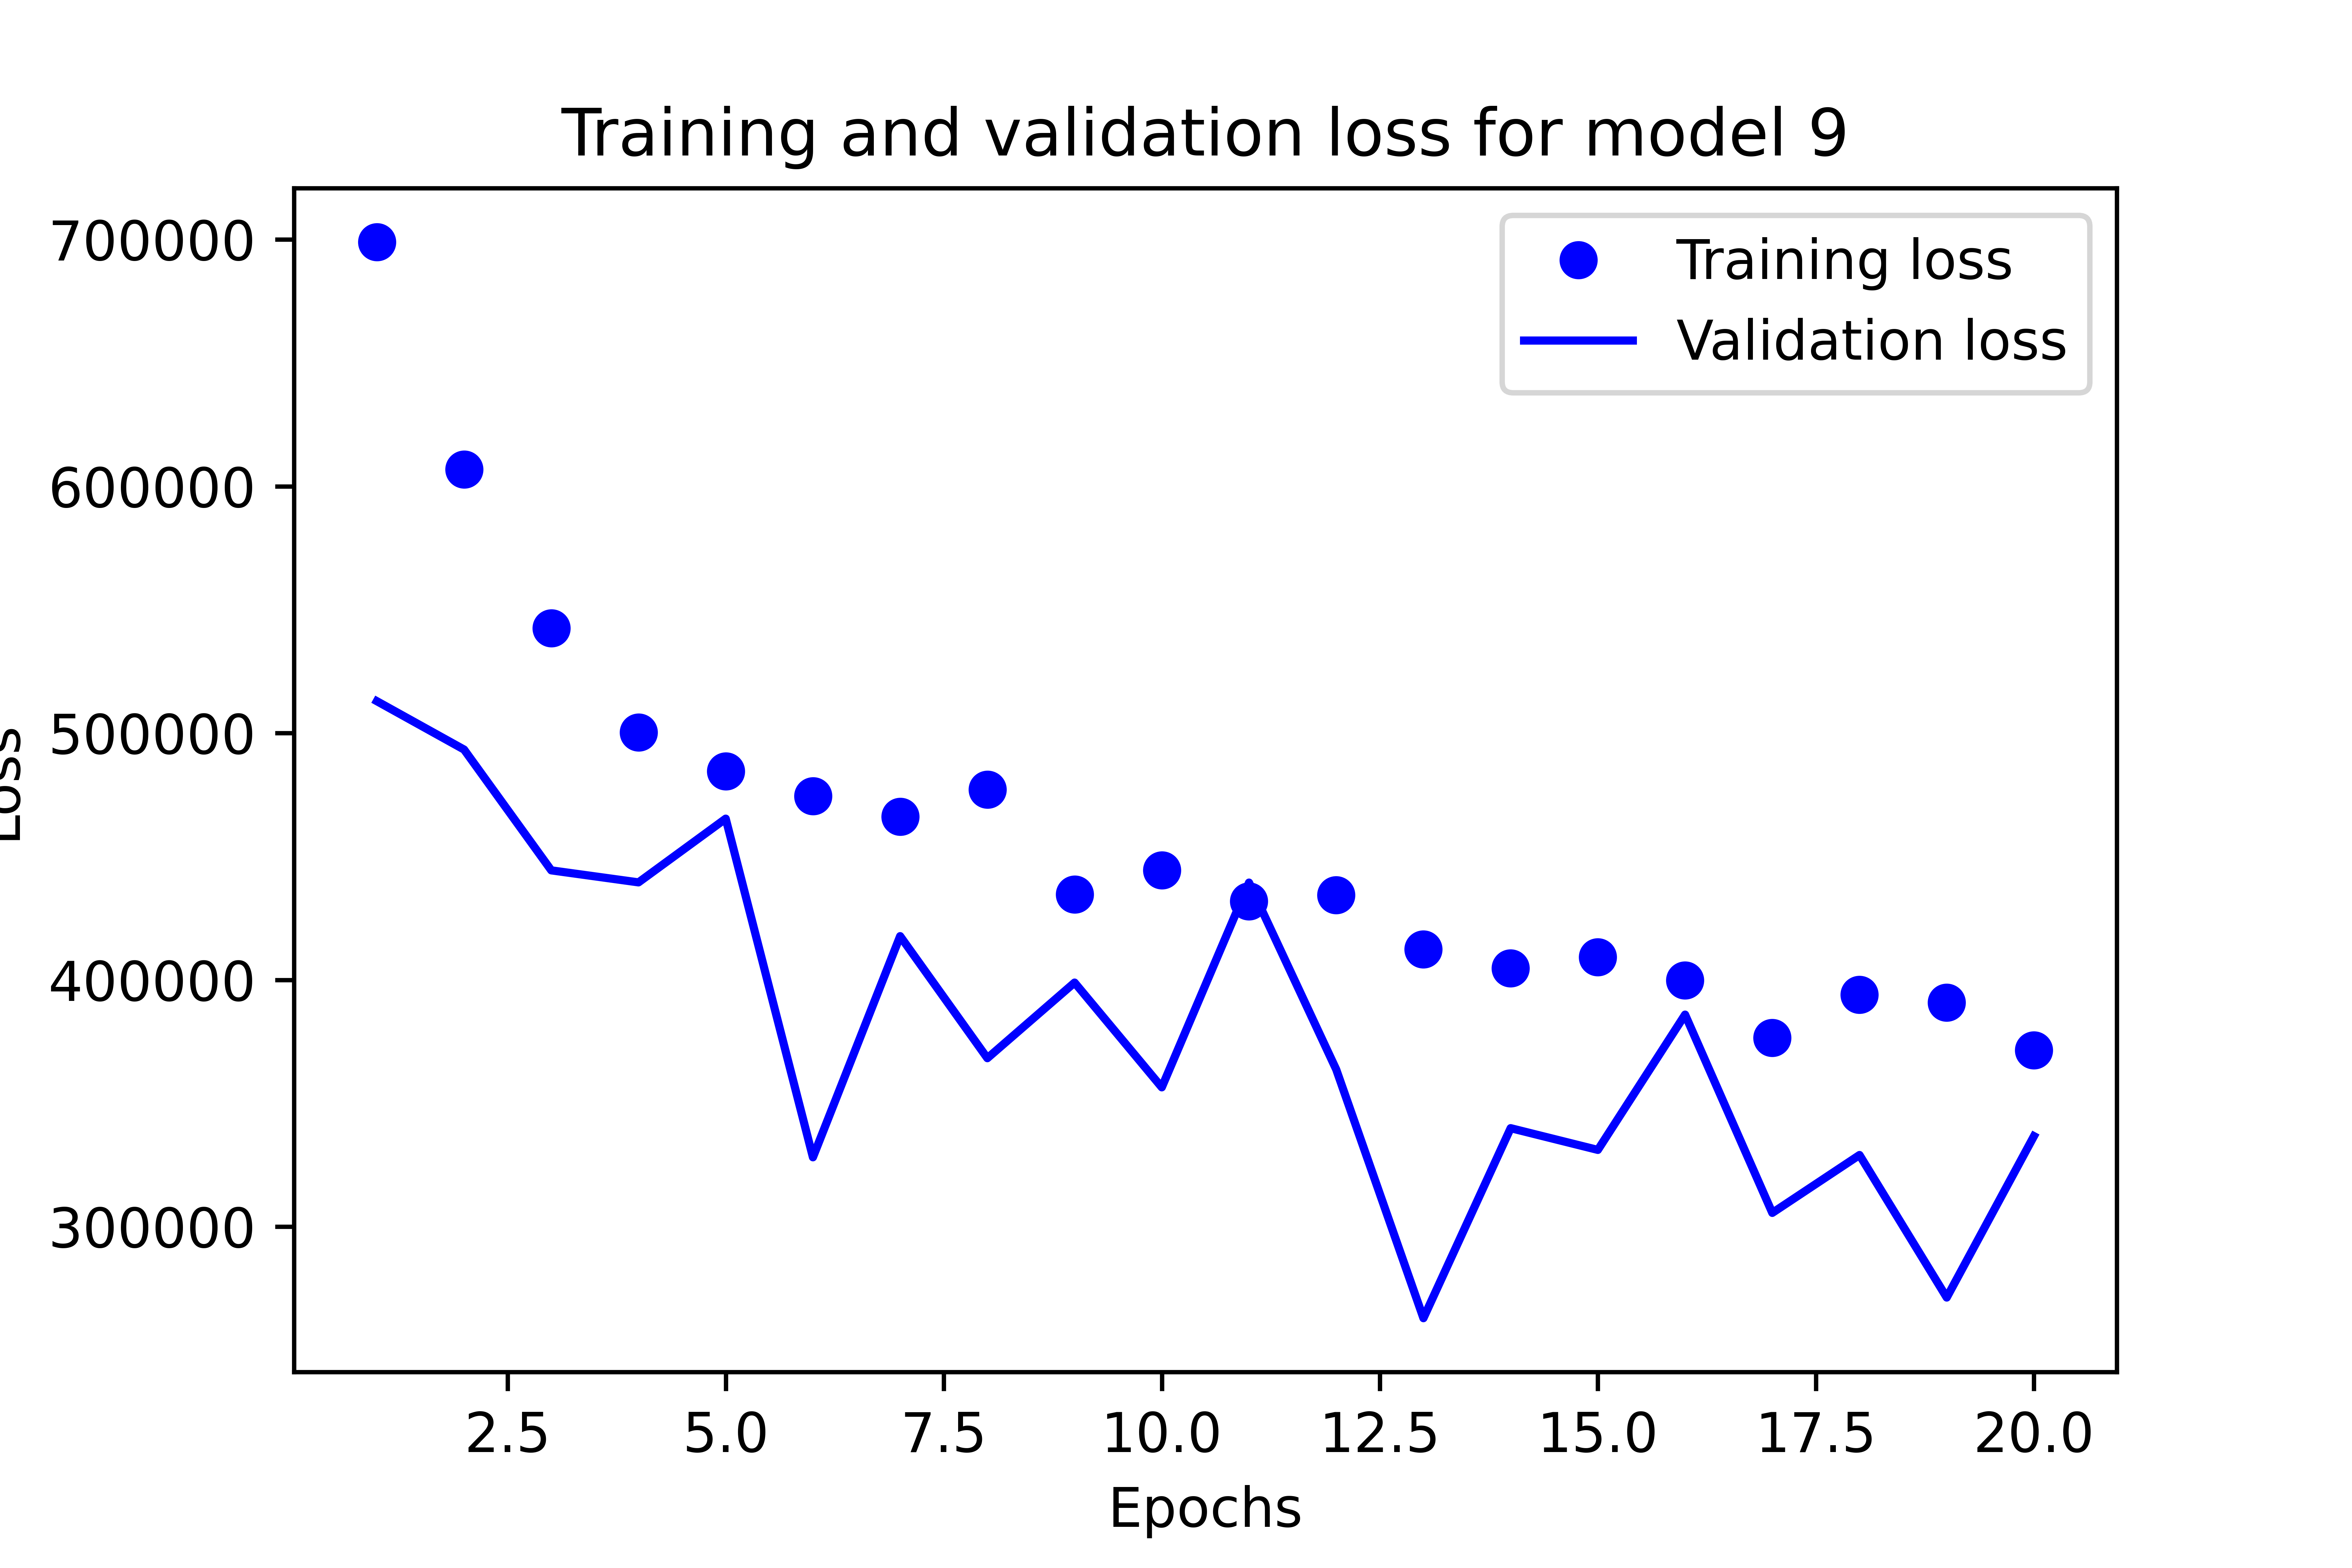
\includegraphics[width=\linewidth]{images/model9.png}
    \end{figure}
    The incremental additions to the model seemed to work, so model 9 added 2 more layers, creating a 128-64-32-16-4-1 structure. 
    This was more radical that the previous iterations because it added hidden layers in the front and the back at the same time. 
    The performance was not good compared to model 8 and the overall increase in loss and validation loss spikes returned.

    \begin{figure}[H]
        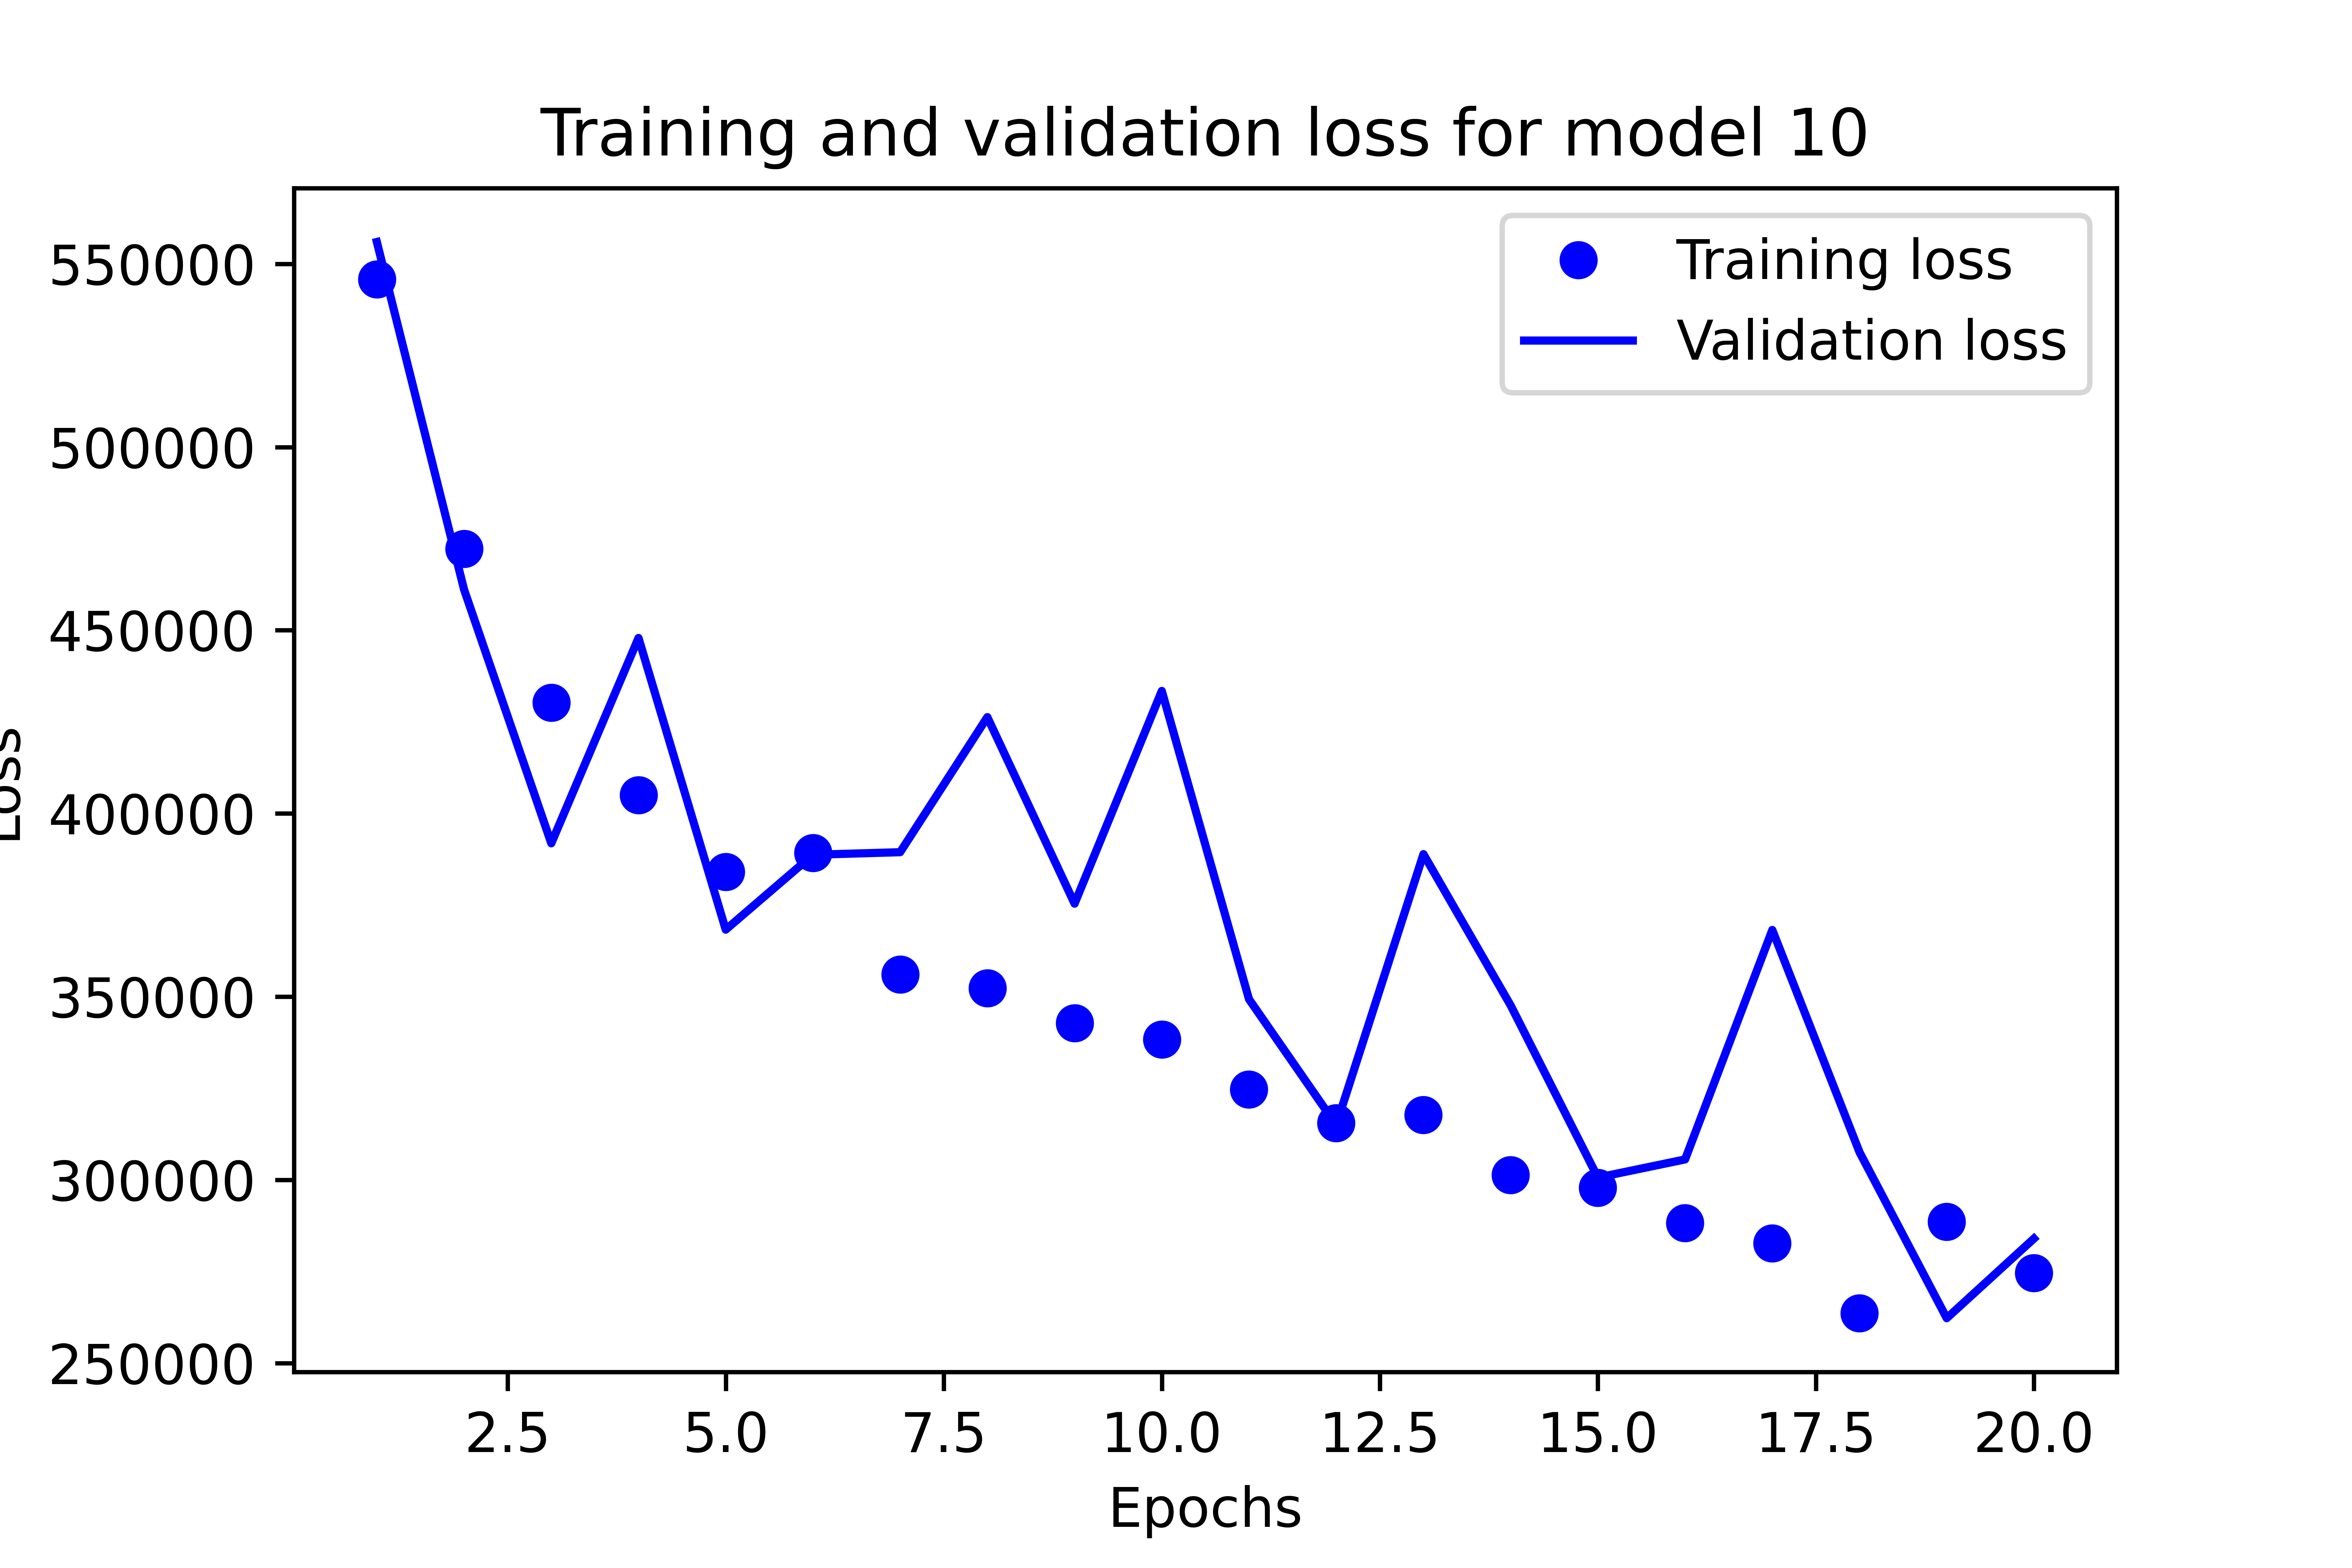
\includegraphics[width=\linewidth]{images/model10.png}
    \end{figure}
    Model 10 was used to test whether if model 9's deficiencies could be fixed with a higher batch size, but this was not the case 
    and the loss got worse. 

    \begin{figure}[H]
        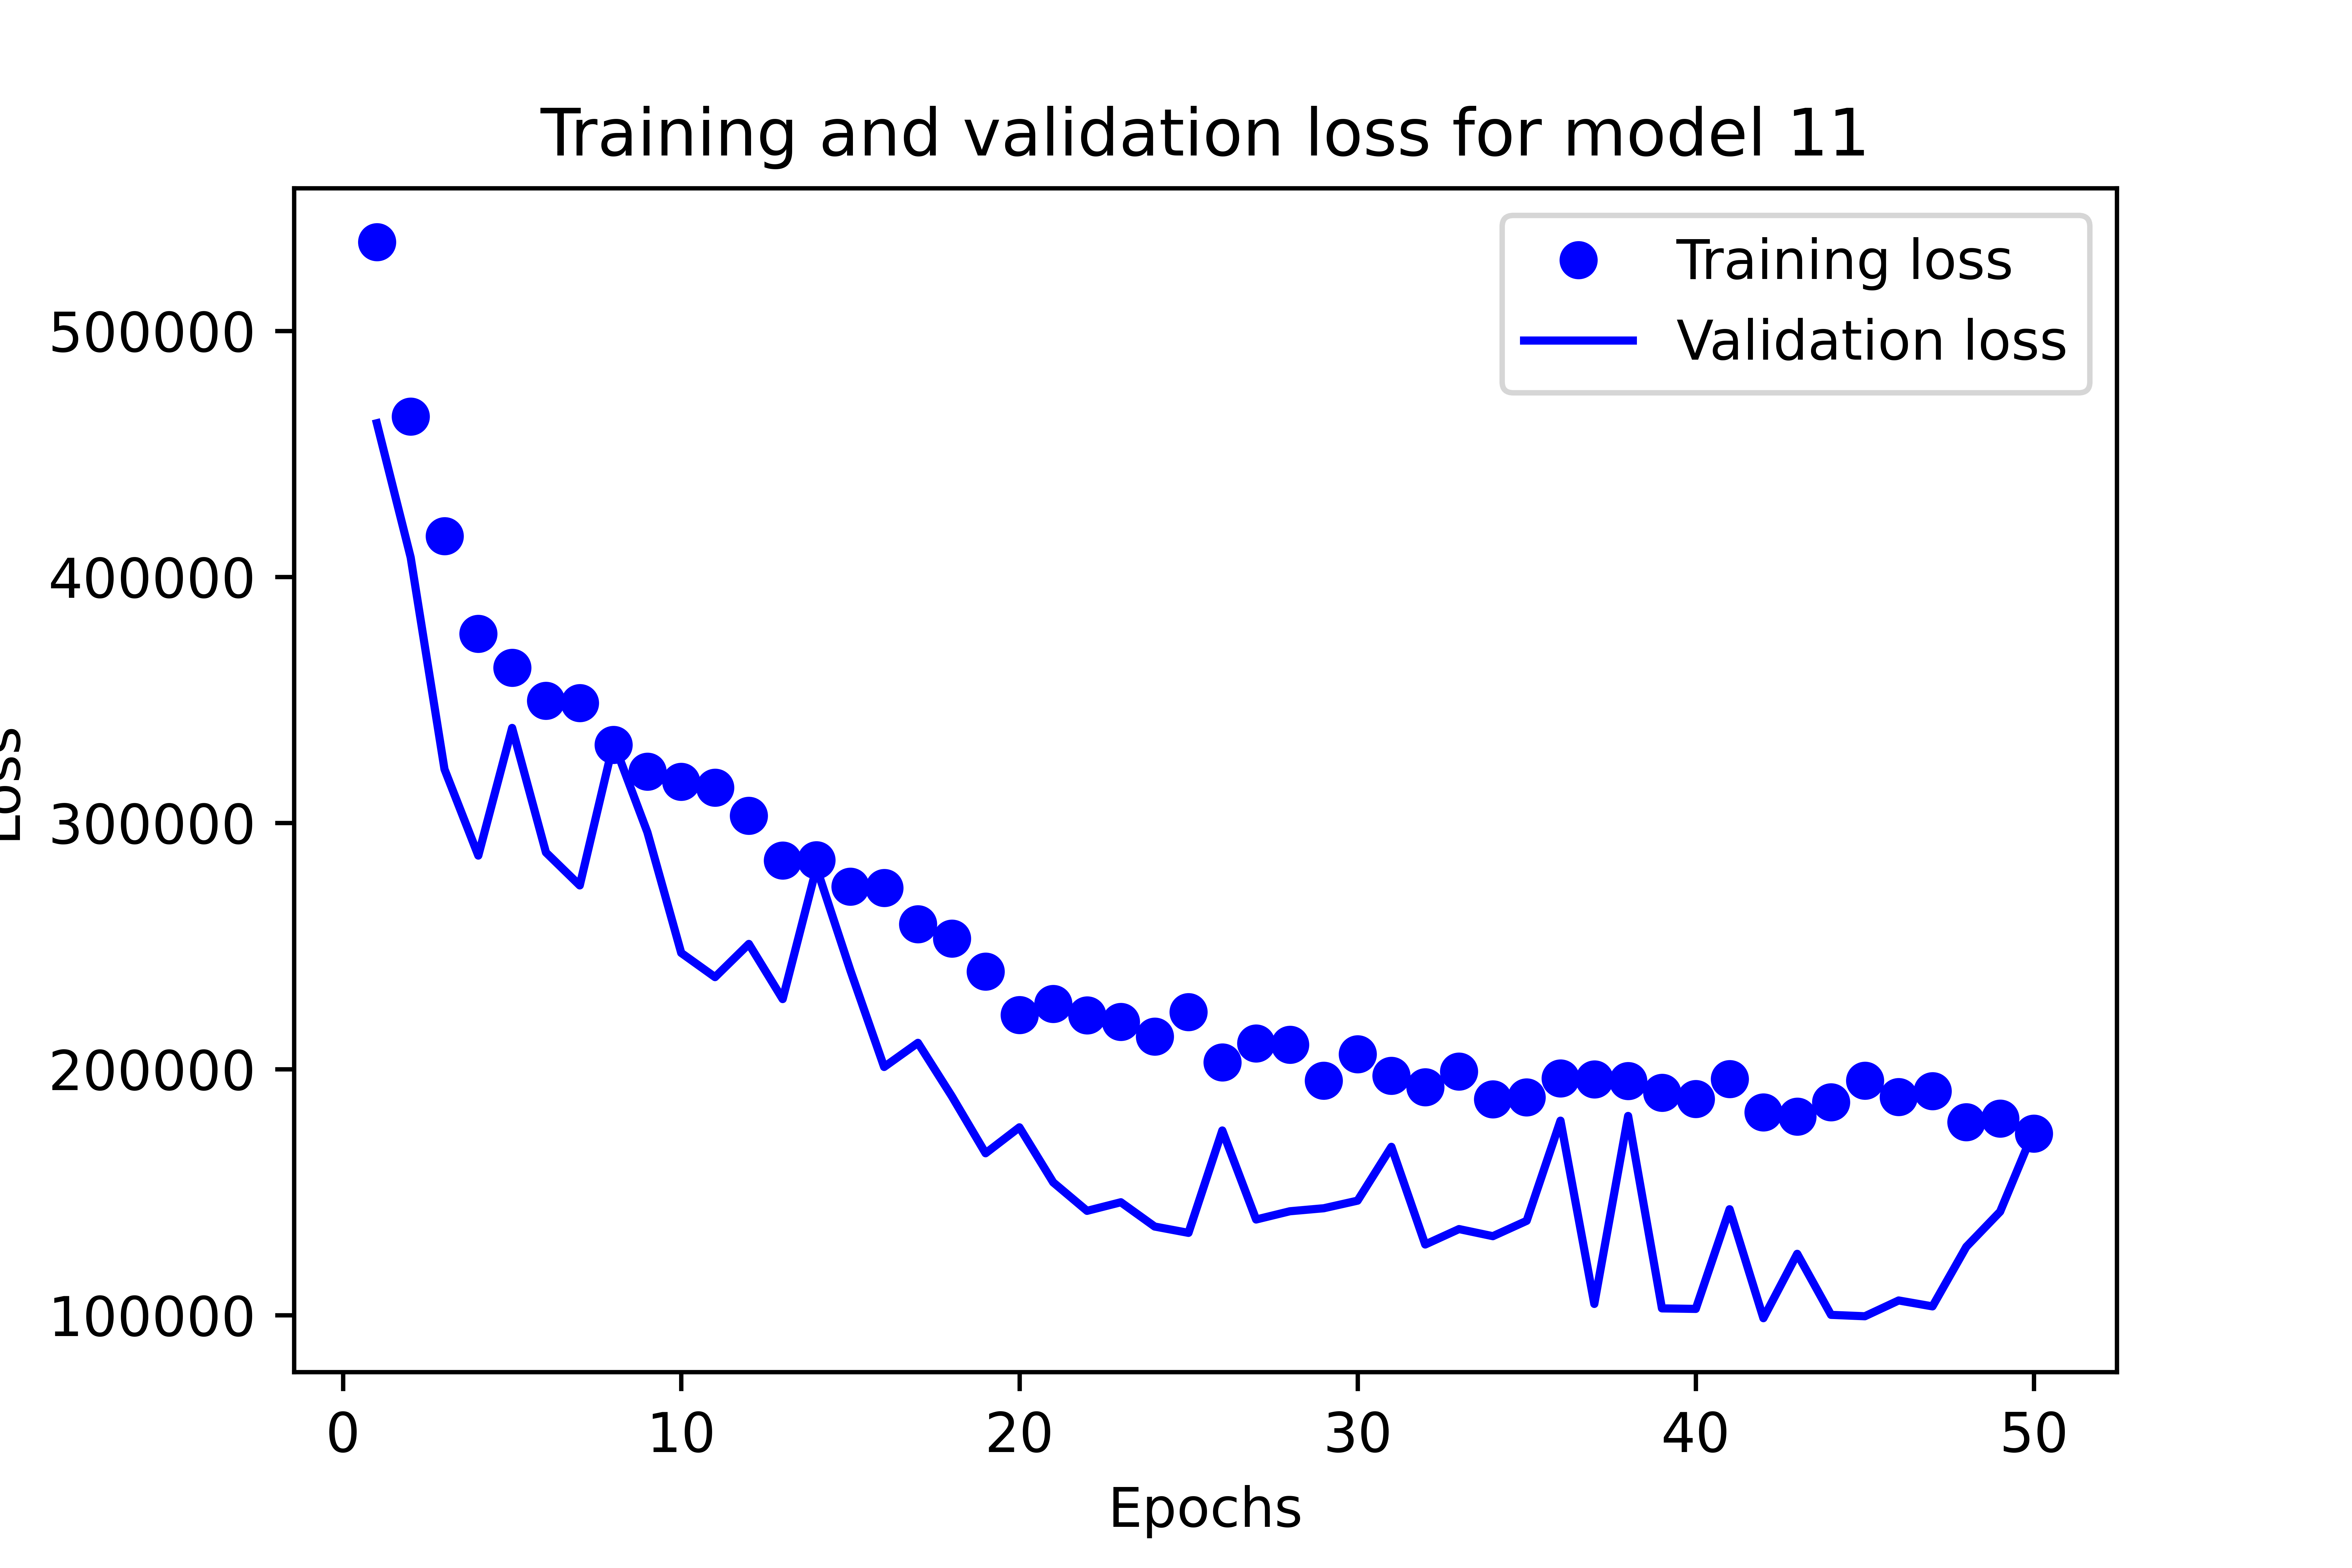
\includegraphics[width=\linewidth]{images/model11.png}
    \end{figure}
    Model 11 went back to the more successful model 8 (with a batch size of 20 and a 64-32-16-8-1 structure), but the 
    number of epochs the model took to train increased from 20 to 50. The purpose was to see if longer training 
    could improve performance by a big margin or whether the model was stuck with the performance of the current model. 
    50 epochs was a relatively good point to stop training because the model started to see diminishing returns around 
    that point and the loss went down significantly compared to epoch 20, but the model found it's limit at epoch 50.

    \begin{figure}[H]
        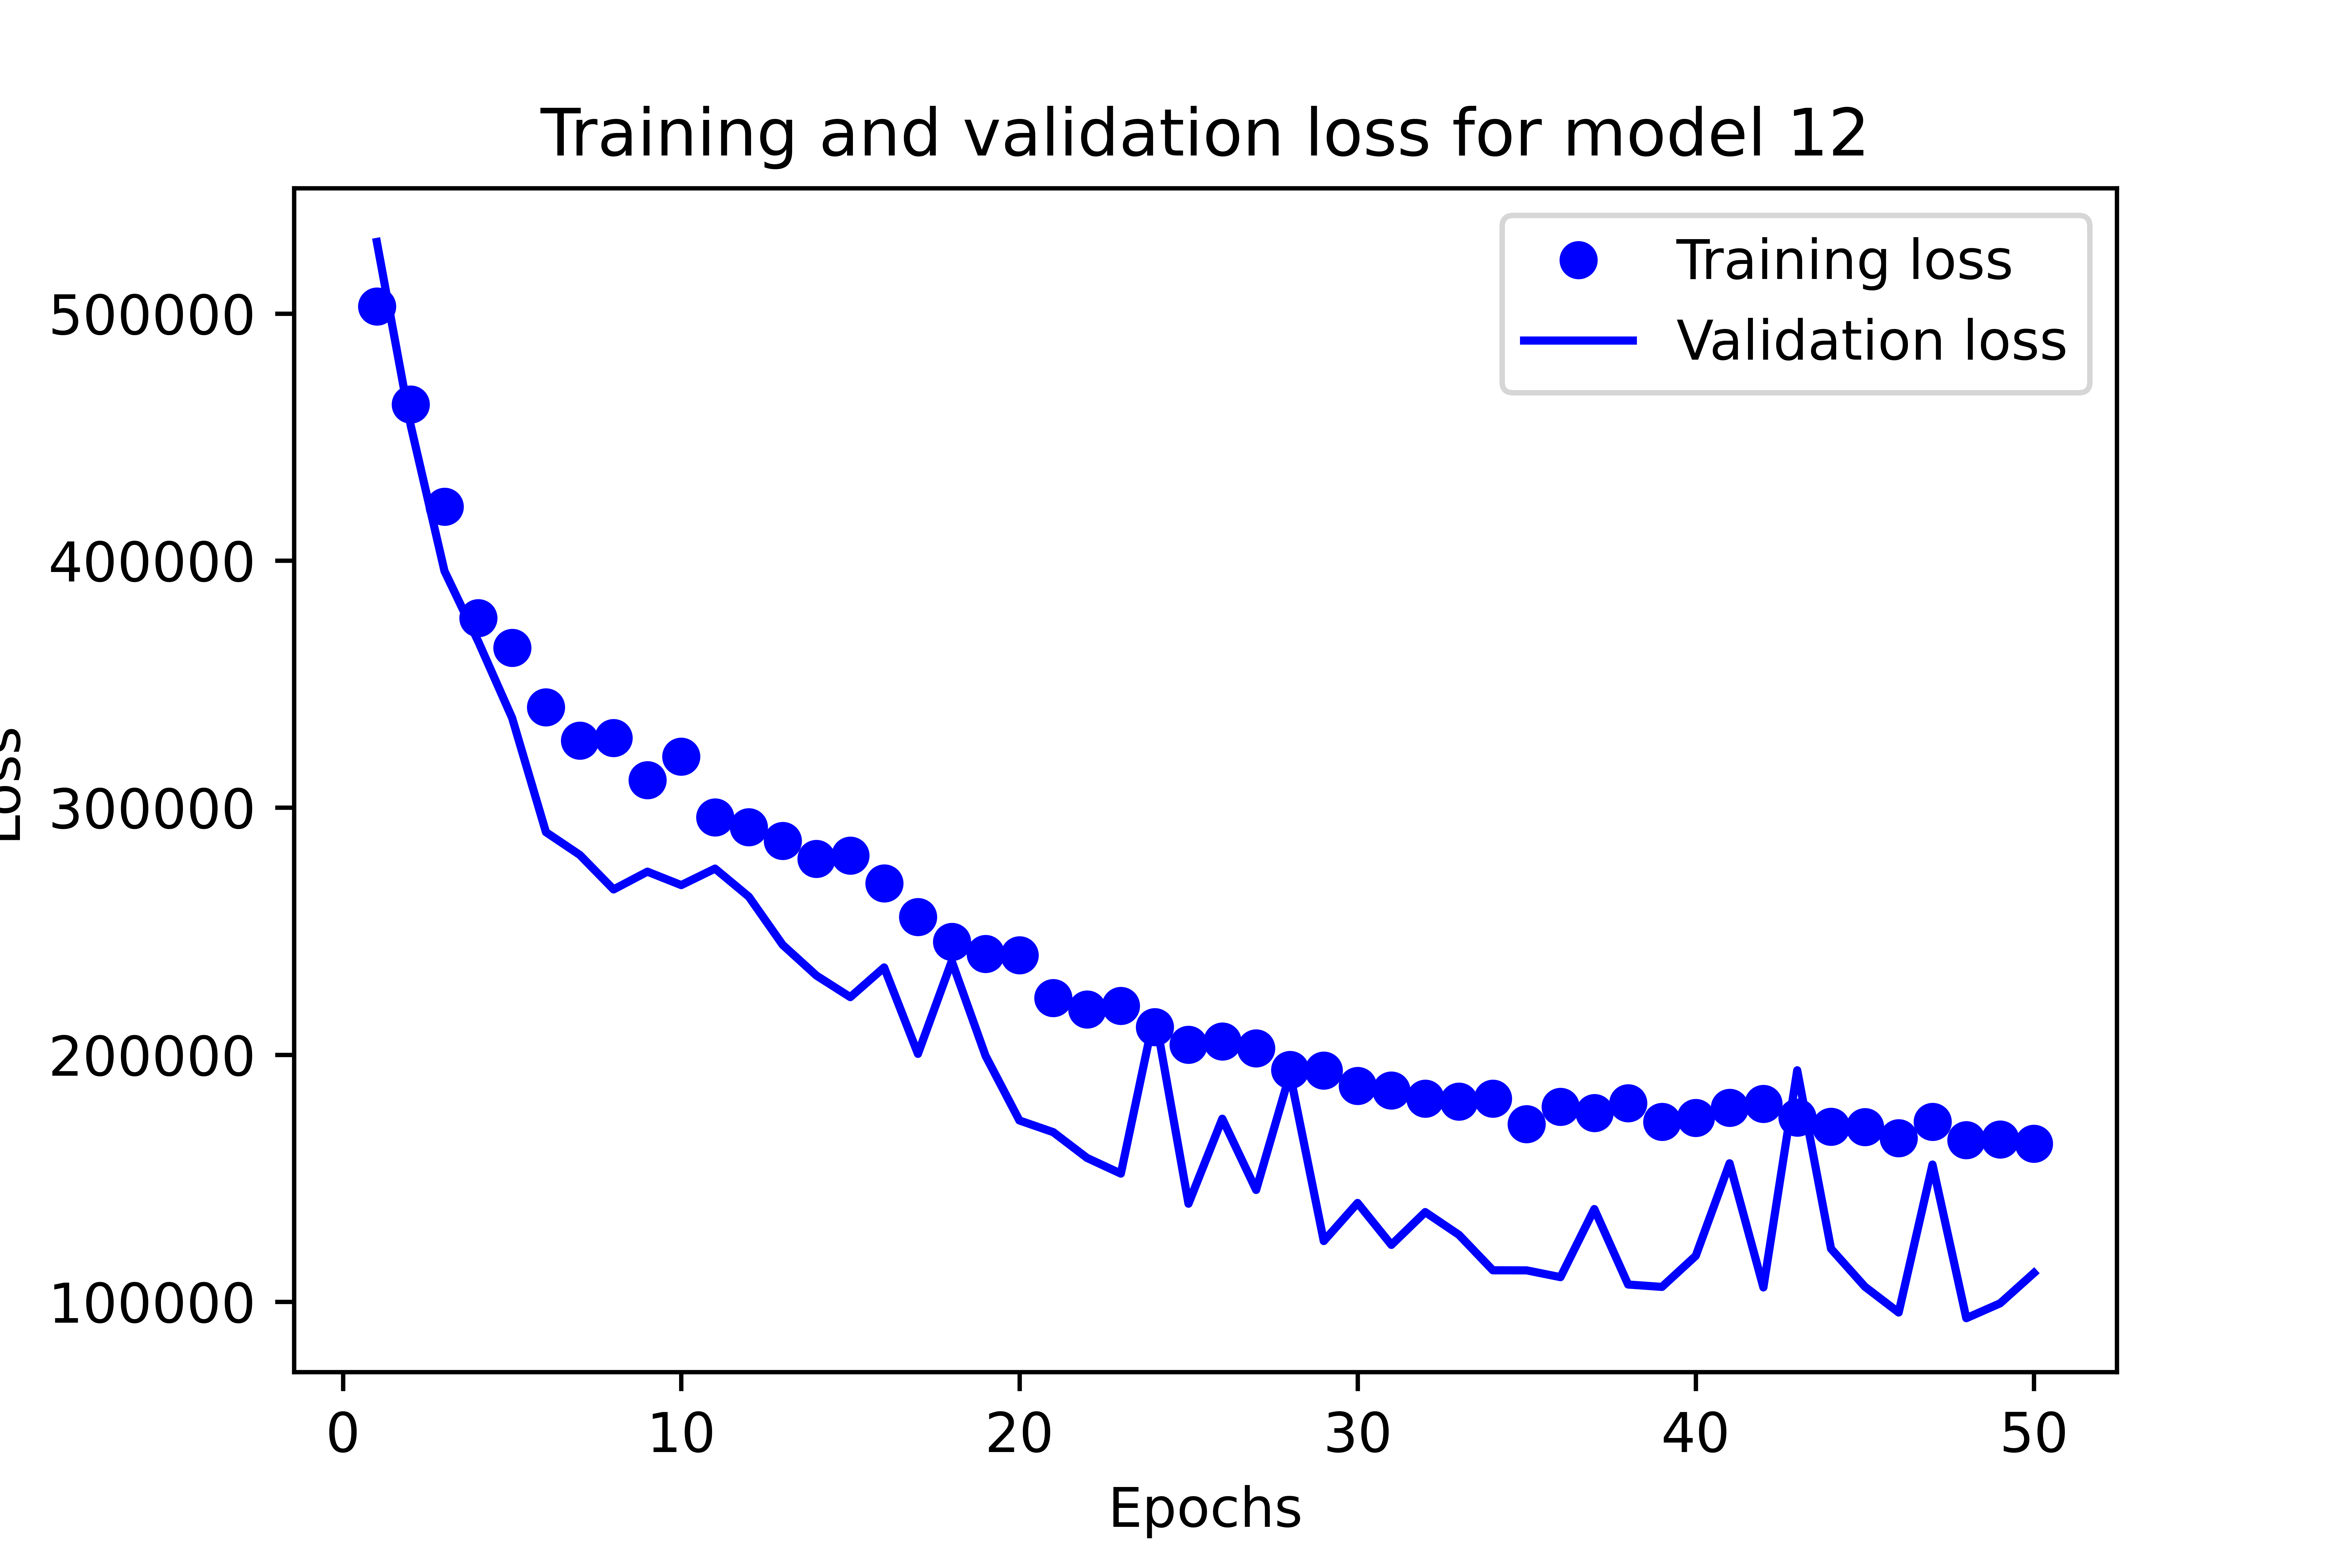
\includegraphics[width=\linewidth]{images/model12.png}
    \end{figure}
    Model 12 tried to improve model 11 by increasing the generalizability and increasing the batch size to 30. This model 
    again achieved a very low overall loss with the validation loss being lower than the training loss. This was about the 
    best the model got in terms of achieving the lowest validation loss even though the loss was still pretty big at around 10,000.

    Other attempts in modifying model 12 ended in about the same or worse performance so this model seems like the best performer 
    that this analysis found. Other methods like increasing batch size to 100, adding a kernel regularizer to each dense layer, 
    and adding layers all resulted in a lower performing model.

\section{Analysis}
    \begin{figure}[h!]
        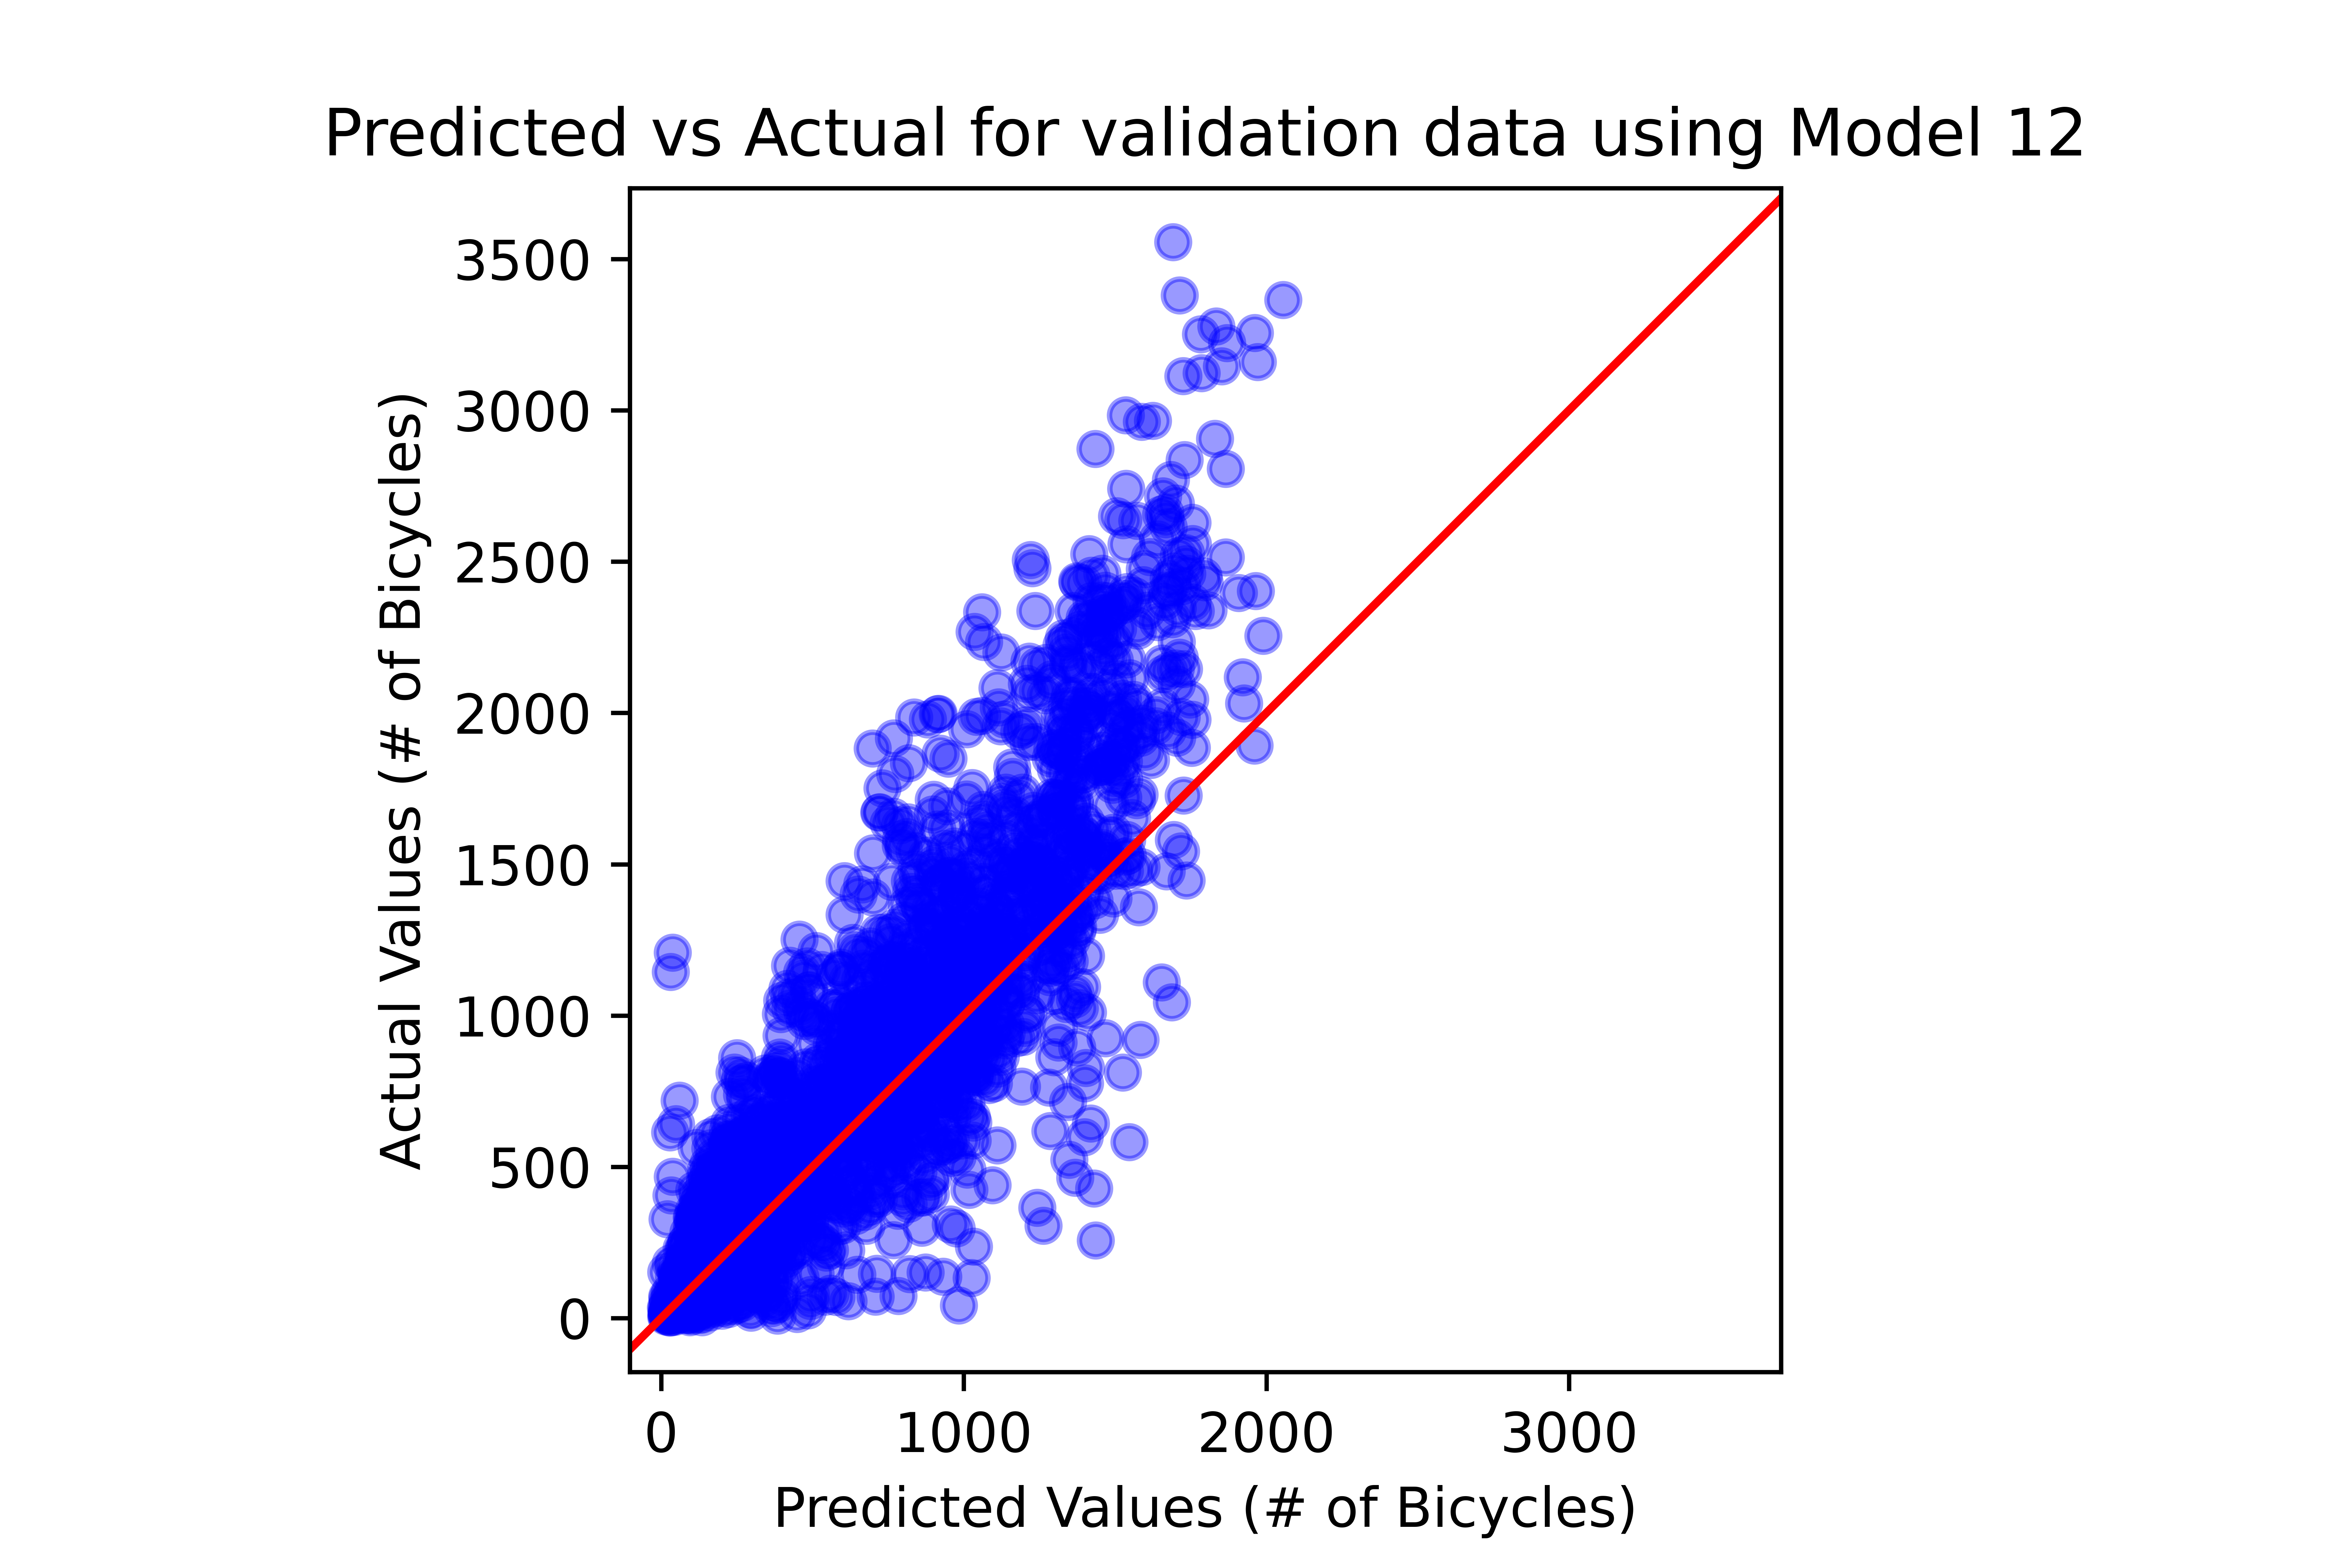
\includegraphics[width=\linewidth]{images/predictactual.png}
        \caption{Predicted v.s. Actual}
        \label{fig:predictactual}
    \end{figure}
    Figure \ref{fig:predictactual} shows the how the predicted value of the number of bicycles rented and the actual number of bicycles rented compare 
    using model 12 to predict the predicted values. 
    The ideal situation is to have all the points on the red line to imply that the model correctly predicted all the actual numbers correctly.
    This is not the case, but the distribution around the line seems even which is a good sign. Also another observation is that there are 
    significantly more data points near the bottom left then fade out towards the top right. This means that there is some imbalance in the dataset.

    \begin{figure}[h!]
        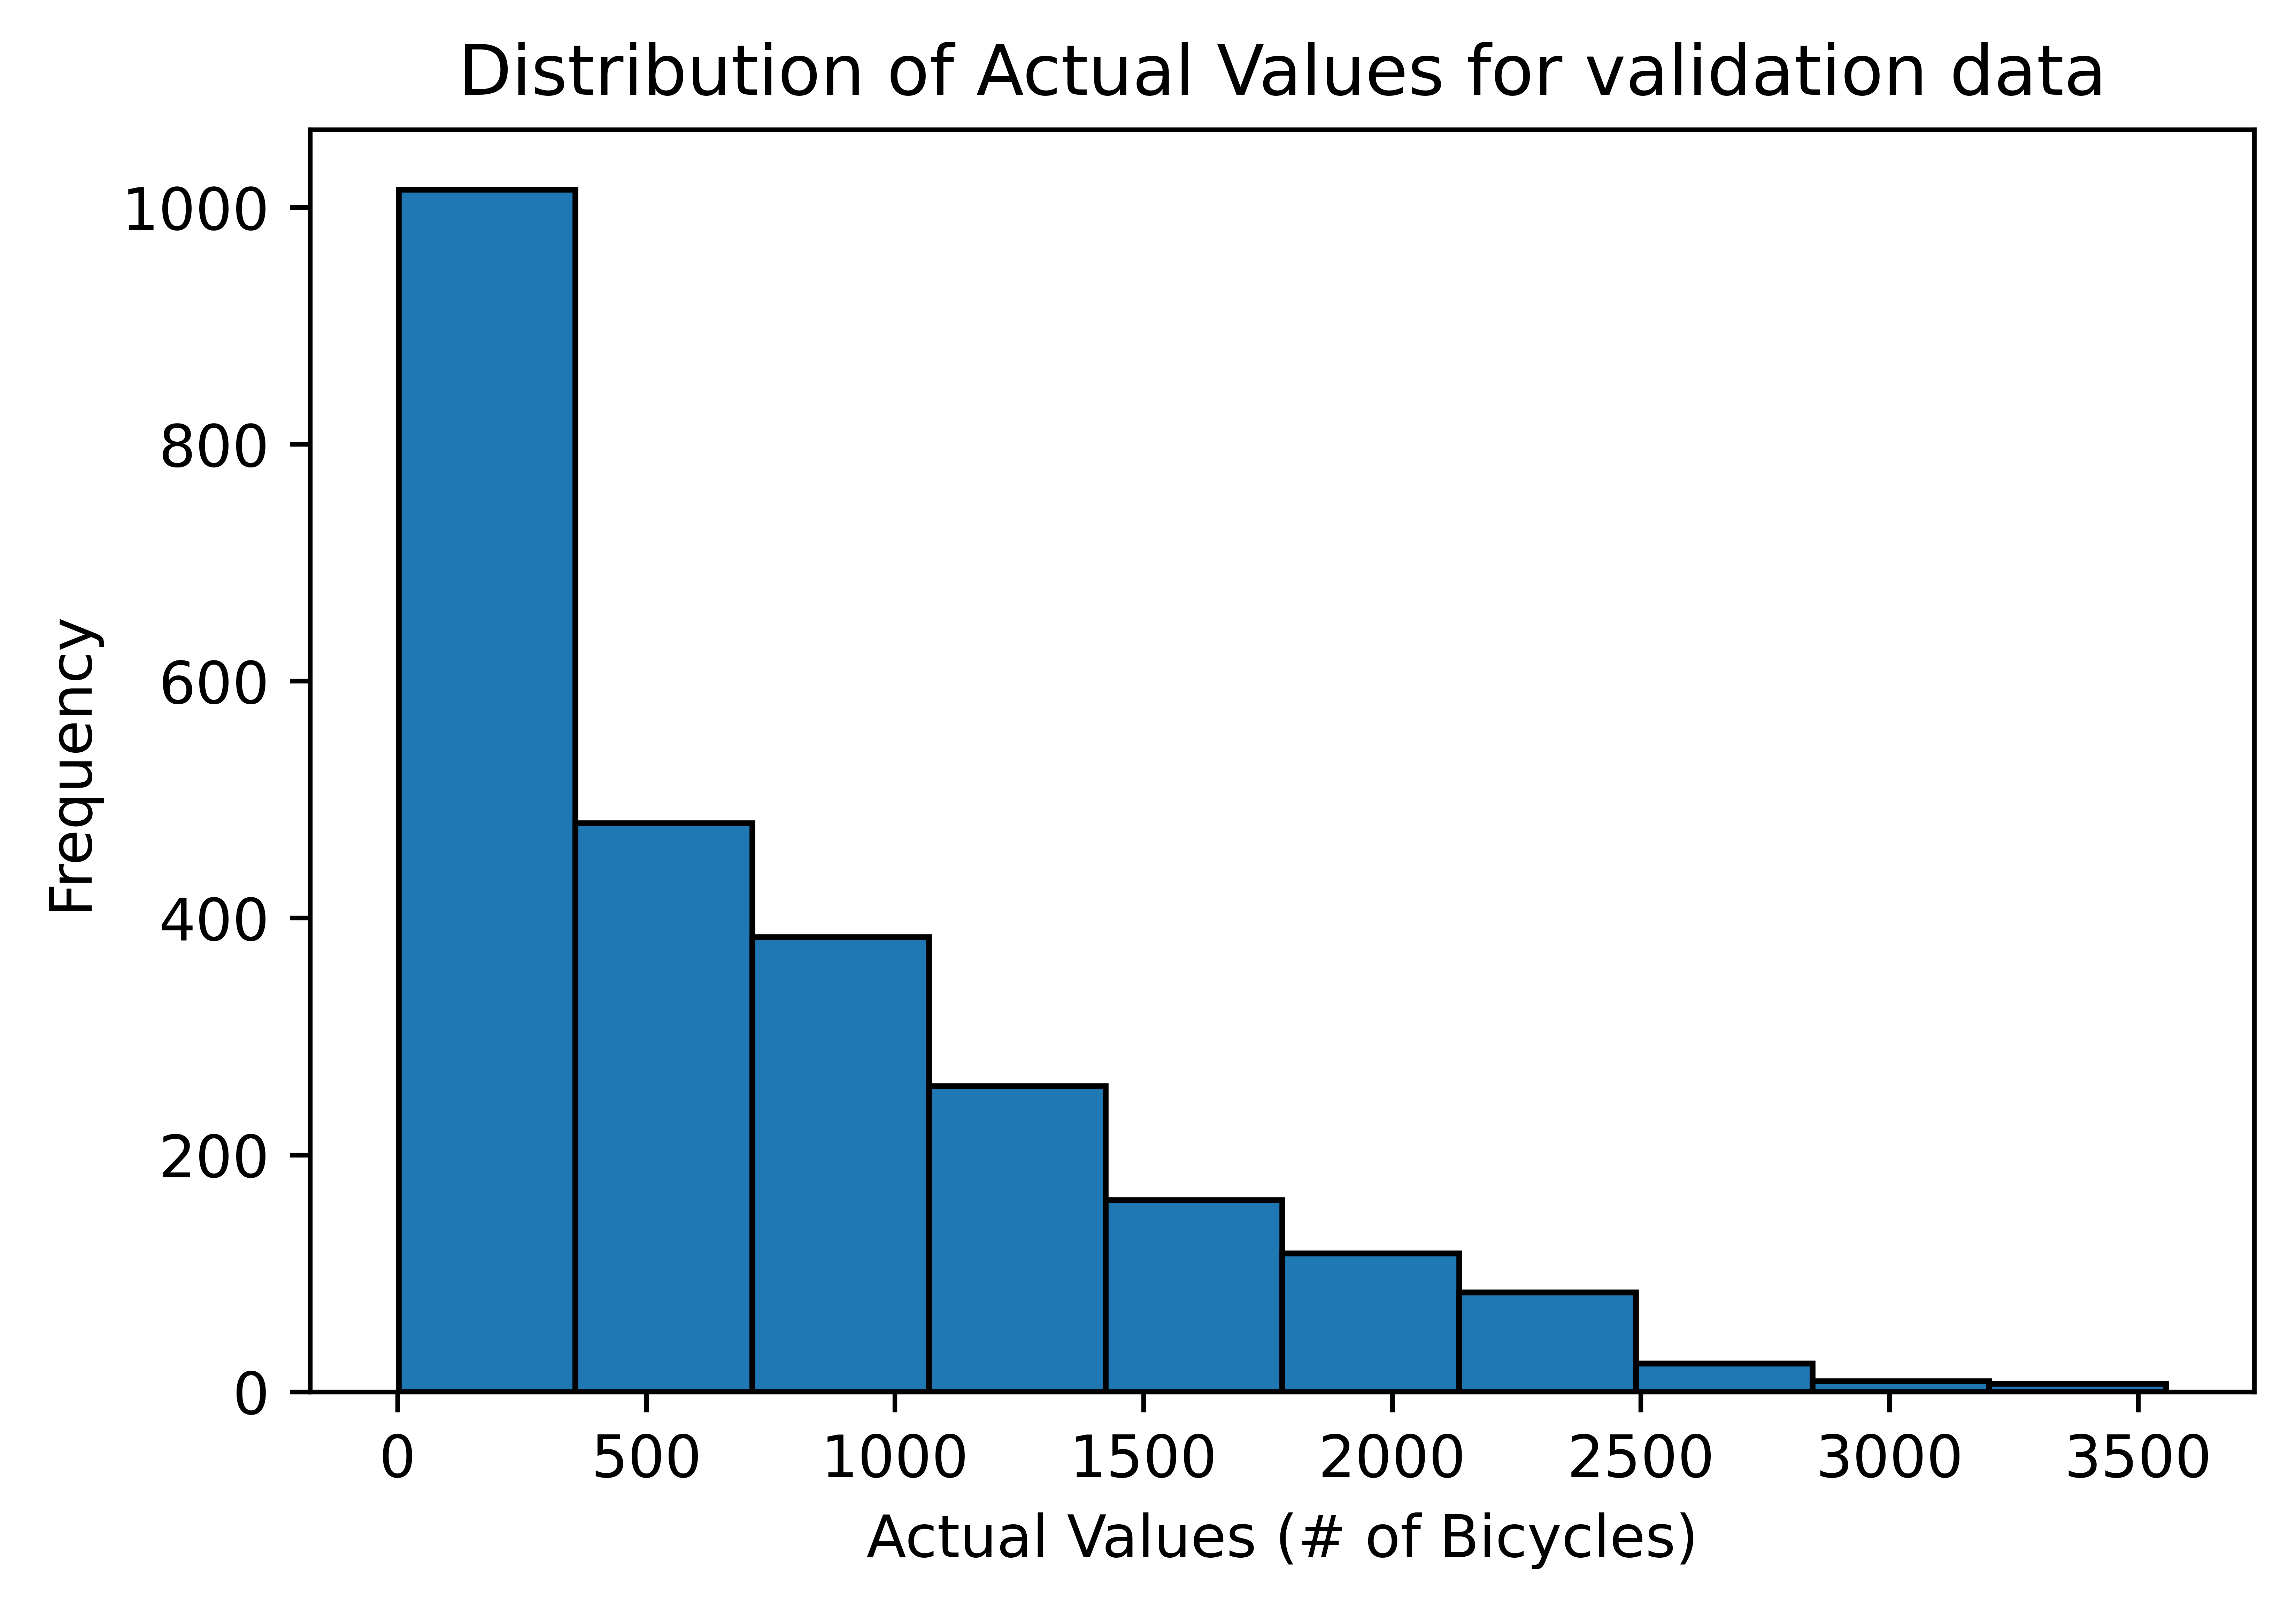
\includegraphics[width=\linewidth]{images/histo.png}
        \caption{Data Distribution}
        \label{fig:histo}
    \end{figure}
    Figure \ref{fig:histo} shows the imbalance in the dataset. There are much more lower number of rented bikes than higher number of rented bikes.
    This might be due to some external factors like weather condtions but also might represent that there is a strong base of 
    renters that use the service often with some of the users only renting once in a while. This also can explain why the model underperformed 
    in certain cases where there were less data points to train on in certain areas of the data, especially the lower frequency data points. 
    The model might also be skewed to predict the higher frequency points with higher accuracy than lower frequency points.

    \begin{figure}[h!]
        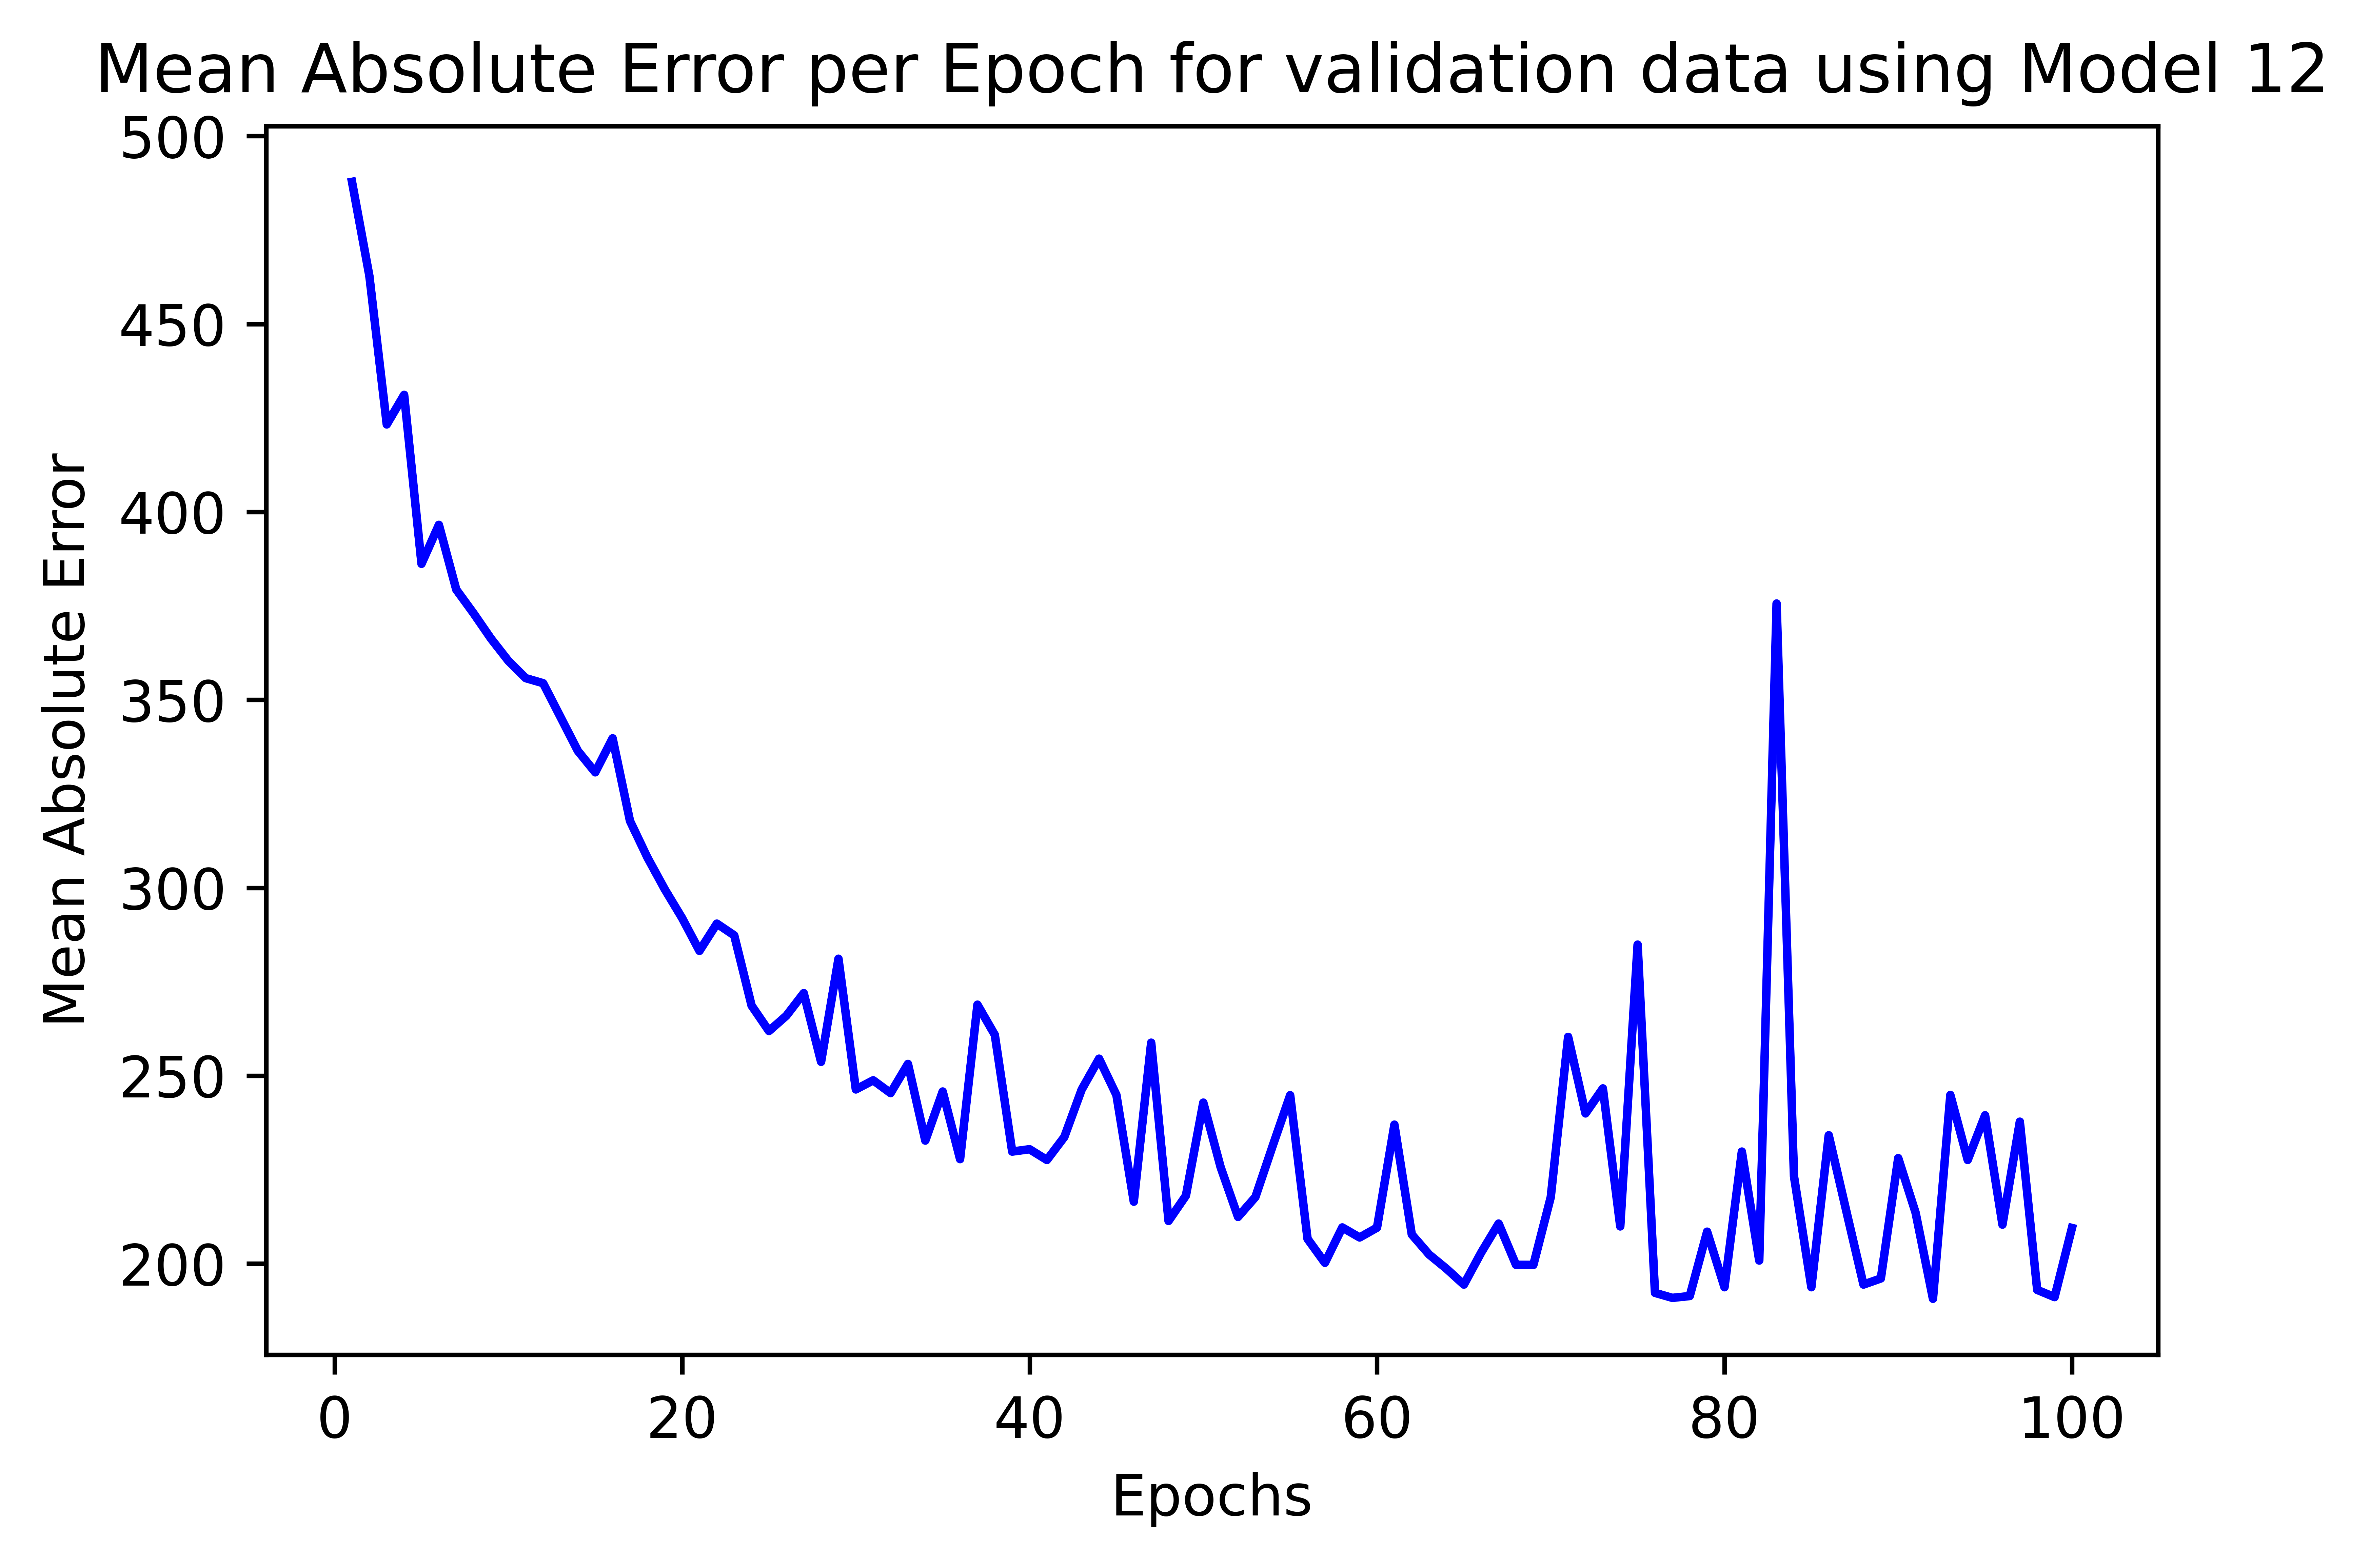
\includegraphics[width=\linewidth]{images/mae.png}
        \caption{Mean Absolute Error}
        \label{fig:mae}
    \end{figure}

    Figure \ref{fig:mae} shows the mean average error for model 12 with the validation data across the epochs. There is a point that the mae 
    meets where the model cannot generalize on new data.

\section{Conclusion}
    The model using the Seoul Bicycle Sharing dataset was moderately able to predict the general number of people who would be renting a bicycle 
    at a certain time. Since this is a seasonal time series dataset, it would also be interesting to compare to other methods where the time 
    dimension can be preserved better.




\end{document}